
\documentclass[a4paper,11pt]{article}

%%%%%%%%%% EXACT 1in MARGINS %%%%%%%                                   %%
\setlength{\textwidth}{6.5in}     %%                                   %%
\setlength{\oddsidemargin}{0in}   %% (It is recommended that you       %%
\setlength{\evensidemargin}{0in}  %%  not change these parameters,     %%
\setlength{\textheight}{9in}      %%  at the risk of having your       %%0
%\setlength{\topmargin}{0.5in}       %%  proposal dismissed on the basis  %%
\setlength{\headheight}{-0.4in}      %%  of incorrect formatting!!!)      %%
\setlength{\headsep}{0.1in}         %%                                   %%



%% Packages for Graphics & Figures %%%%%%%%%%%%%%%%%%%%%%%%%%
\usepackage{graphicx}
\usepackage{url}
\usepackage{csquotes}
\usepackage[labelsep=endash, figurename=Figure, tablename=Table, textfont=it]{caption}
\usepackage{subcaption}
\usepackage{float}  
\usepackage{hyperref}
\usepackage{multicol}
\usepackage{multirow}
\usepackage{tikz}

%% Other Packages %%%%%%%%%%%%%%%%%%%%%%%%%%%%%%%%%%%%%%%%%%%
\usepackage{fancyhdr}
\usepackage[top=2.5cm, bottom=2.5cm, left=2.5cm, right=2.5cm]{geometry} 
\usepackage[usenames,dvipsnames]{pstricks}
\usepackage[round,comma,authoryear]{natbib}
\usepackage{titling}
\usepackage{amsmath,amssymb, mathtools,authblk, amsthm}
\usepackage[dvipsnames]{xcolor}
\usepackage[sc]{mathpazo} 
\linespread{1.05}
\usepackage{comment}

\usepackage{booktabs}

% %%%%%%%%%%%%%%%%%%%%%%%%%%%%%%%%%%%%%%%%%%%%%%%%%%%%%%%%%%%%%
% %% Options / Modifications
% %%%%%%%%%%%%%%%%%%%%%%%%%%%%%%%%%%%%%%%%%%%%%%%%%%%%%%%%%%%%%
\definecolor{darkblue}{rgb}{0,0,0.5}
\hypersetup{colorlinks=true,linkcolor=black,citecolor=darkblue,urlcolor=darkblue} 
\DeclareMathOperator*{\argmax}{arg\,max}
\DeclareMathOperator*{\argmin}{arg\,min}
\newtheorem{proposition}{Proposition}
\newtheorem*{proposition*}{Proposition}
\newtheorem{theorem}{Theorem}
\newtheorem{lemma}{Lemma}
\newtheorem{definition}{Definition}
\newtheorem{corollary}{Corollary}
\newtheorem{assumption}{Assumption}
\newtheorem{remark}{Remark}
\newcommand{\relint}{\operatornamewithlimits{relint}}
\newcommand{\R}{\mathbb{R}}
\def\tr{\color{red}}
\def\tb{\color{red}}
\newcommand{\io}{ \boldsymbol{\iota} }
\newcommand{\m}{ \mathbf }

\begin{document}

\title{Sensitivity analysis of the\\ perturbed utility stochastic traffic equilibrium\thanks{We are grateful to an anonymous referee for pointing out the connection to the machine learning literature. }}
\author[a]{Mogens Fosgerau\footnote{Corresponding author: \url{mogens.fosgerau@econ.ku.dk}}}
\author[a]{Nikolaj Nielsen}
\author[b]{Mads Paulsen}
\author[b]{Thomas Kjær Rasmussen}
\author[c]{Rui Yao}
\affil[a]{University of Copenhagen, Denmark}
\affil[b]{Technical University of Denmark, Denmark}
\affil[c]{EPFL, Switzerland}
\date{\today}
\maketitle

\begin{abstract}
This paper develops a novel sensitivity analysis framework for the perturbed utility route choice (PURC) model and the accompanying stochastic traffic equilibrium model. We provide general results that determine the marginal change in link flows following a marginal change in link costs across the network in the cases of flow-independent and flow-dependent link costs. We derive analytical sensitivity expressions for the Jacobian of the individual optimal PURC flow and equilibrium link flows with respect to link cost parameters under mild differentiability assumptions.
Numerical examples illustrate the robustness of our method, demonstrating its use for estimating equilibrium link flows after link cost shifts, identifying critical design parameters, and quantifying uncertainty in performance predictions. The findings have implications for network design, pricing strategies, and policy analysis in transportation planning and economics, providing a bridge between theoretical models and real-world applications. 

\end{abstract}

\bigskip

\noindent \textbf{Keywords:} Sensitivity analysis; perturbed utility; route choice; stochastic traffic equilibrium


\section{Introduction}

The novel perturbed utility route choice (PURC) model \citep{Fosgerau2021a,fosgerau_bikeability_2023}, and the corresponding traffic equilibrium model \citep{yao_perturbed_2024} have several attractive features, deriving from the fact that the PURC model predicts the behavior of an individual traveler simply as link flows across a network, and not as a probability distribution over paths. This allows the model to include the whole network, thus avoiding choice set generation and its associated difficulties. The PURC model allows zero flows on irrelevant parts of the network to be predicted, adding behavioral realism to the classical discrete route choice models. 

An additional attractive feature is that the dependence of predicted link flows on link costs throughout the network follows from the structure of the network. In this paper, we are concerned with estimating this dependence. In other words, we are concerned with sensitivity analysis.

Sensitivity analysis is central to bilevel optimization problems, e.g., network design and pricing problems \citep{yang1997traffic,josefsson2007sensitivity}, (hyper)parameter optimization and meta-learning \citep{franceschi2018bilevel,lorraine2020optimizing}, as well as deep equilibrium and implicit models \citep{bai2019deep}. Sensitivity analysis is challenging in the PURC setting since we use the complete network as the choice set and allow every path to be considered. Consequently, changes in an attribute on a link can nontrivially impact the optimal flows on other links through the network structure. %This could bring significant computational challenges to the bilevel problems. 

Many existing additive random utility (ARUM, \cite{mcfadden_econometric_1981}) route choice models impose simplifying assumptions that reduce the complexity of sensitivity analysis. For example, the application of path-based route choice models often only considers a subset of pre-generated paths~\citep{vovsha_link-nested_1998,duncan2020path}, which may lead to bias, also in the sensitivity analysis. 
In addition, ARUM route choice models predict, by design, a strictly positive choice probability for every path alternative in the choice set. Hence, the predicted probability vector is always interior in the probability simplex, which allows simple implicit function-based sensitivity analysis methods to be applied~\citep{tobin1988sensitivity}.

In contrast, this paper studies sensitivity analysis in a more general setting, where all paths in the complete network are considered, and zero flows on irrelevant parts of the network are allowed. We consider sensitivity analysis for both the cases of flow-independent and flow-dependent link costs.
The first main contribution of this paper is Theorem \ref{thm:jacobian}, which gives a computationally efficient analytical expression for the sensitivity of optimal link flows with respect to the parameters in the flow-independent link cost functions. 
We then extend the analytical sensitivity analysis to the flow-dependent case in Theorem \ref{prop:jacobian_equilibrium_cost}, our second main contribution. This result applies to the sensitivity analysis of traffic equilibrium. 
Notably, our analytical sensitivity expressions hold for the whole PURC model family under similar differentiability conditions as in~\cite{patriksson_sensitivity_2004}. 

A particular finding, illustrated with examples, is that some pairs of paths can be complements in the PURC model. This contradicts a result in a previous paper in this journal; we point out and correct the error.

We illustrate our theoretical results in a prediction of equilibrium link flow patterns following changes in network parameters while avoiding having to resolve for equilibrium. We also show how sensitivity results can assist in the uncertainty analysis of prediction outputs when there are uncertainties in network parameters.


\subsection{Literature review}
\subsubsection{Sensitivity analysis and route choice substitution patterns }
Sensitivity analysis in the route choice context concerns estimating the changes in travelers' route choice decisions following changes in the utilities or attributes of alternatives. This is also termed as a \textit{substitution pattern} in the demand modeling literature. It sheds light on substitution and complementarity relationships between choice alternatives, which consequently can be used to inform policy and decision-making~\citep{ben1985discrete}. 

Sensitivity analysis for classical route choice models can be obtained by deriving the Jacobian of the route choice probabilities with respect to utilities or attributes, provided that the route choice probabilities satisfy specific differentiability conditions~\citep{robinson_strongly_1980, robinson1985implicit}. This is the case for most route choice models in the literature that belong to the ARUM family. 
A common feature of ARUM is that its choice probability function exists and is continuously differentiable in utilities~\citep{mcfadden_econometric_1981,Fosgerau2013y}. When the choice probability function is available in closed form, this allows the substitution pattern to be obtained directly by differentiation. %For example, it reveals the well-known drawback of multinomial logit model (MNL), the independence of irrelevant alternatives (IIA) property~\citep{Luce1959a}, namely, a cost increase on one path causes demand to increase on all other paths by the same proportion.

Sensitivity analysis can be useful for developing ARUM route choice models with more plausible substitution patterns. For instance, the probability of choosing a specific path is expected to be more sensitive to cost increases on paths with overlapping links (i.e., closer substitutes) than on other paths. This leads to the development of ARUM-based route choice models that embed the network structure in order to induce such correlations. The path-size logit model~\citep{ben1999discrete} incorporates correlation between alternatives in the systematic part of the utility function. This family of models also includes the generalized path-size logit \citep{ramming2001network}, path-size correction logit~\citep{bovy2008factor}, and adaptive path-size logit~\citep{duncan2020path}. In essence, these path-size logit models assume overlapping paths are more sensitive to changes in each other's selected attributes (e.g., length, time). Consequently, substitution patterns depend on which attributes are changed. 

Another approach accounts for statistical correlation via the ARUM random error term, thus substitution patterns depend on utilities, regardless of which attributes are changed. 
These models can be further categorized into path-based and link-based. Examples of path-based generalized extreme value (GEV) models include link-nested logit~\citep{vovsha1997application,bekhor1999formulations, marzano2008covariance}, generalized nested logit~\citep{wen2001generalized, bekhor2001stochastic} and paired combinatorial logit~\citep{chu1989paired, bekhor1999formulations, gliebe1999route}. These path-based GEV models typically assume a nesting structure, where path alternatives sharing common links are assigned to the same nest(s) according to predefined rules. Yet, specifying nesting structures can be challenging since many nesting structures are possible, and different nesting structures lead to different substitution patterns. 
Link-based GEV models overcome such challenges by inducing substitution patterns directly from the network structure while assuming travelers sequentially choose the next link at each node. Typical link-based GEV models include the recursive logit model~\citep{fosgerau2013link} and its extensions, the recursive nested logit~\citep{mai2015nested}, and recursive network GEV model~\citep{mai2016method,oyama2019prism} that relax the IIA assumption at the link level. 

Indeed, recursive GEV models~\citep{fosgerau2013link, mai2015nested, mai2016method,oyama2019prism} are similar to the PURC model~\citep{Fosgerau2021a} in the sense that they are both link-based and allow for flexible substitution induced directly by the network structure. One key distinction, however, is that the PURC model allows zero flows in irrelevant parts of the network, while recursive GEV models assign strictly positive choice probabilities on every link. This feature, on the other hand, brings additional complexity for sensitivity analysis as typical differentiability conditions in ARUM need not hold in the case of PURC models. Drawing inspiration from \cite{kyparisis1990solution,patriksson_sensitivity_2004}, this paper formulates a differentiability condition for the PURC model family and provides an analytical expression for the sensitivity of optimal PURC flows.

% { Alternative route choice models have recently been proposed that allow implicitly assigning zero choice probability to some alternatives in the choice set (e.g., \cite{WATLING2018, tan_endogenously_2024, Rasmussen2024}). However, in practical implementations, these models still need to consider only a subset of the universal choice set due to the size of the complete network.}

\subsubsection{Sensitivity analysis for traffic equilibrium}
Sensitivity analysis of traffic equilibrium extends sensitivity analysis for route choice to the case where link costs are flow-dependent.
It quantifies the rate of changes in \textit{equilibrium} traffic flows as a function of network parameters.
A key application of traffic equilibrium sensitivity is to estimate the change in equilibrium flow patterns that follows a change in network parameters without having to completely re-solve the traffic equilibrium problems~\citep{tobin1988sensitivity, yang1997traffic, patriksson2003sensitivity}.

Similar to the route choice scenario, sensitivity analysis of traffic equilibrium can be carried out by (generalized) differentiation of the equilibrium link flows with respect to network parameters if certain differentiability conditions hold \citep{robinson1985implicit, robinson2006strong}. In general, if the equilibrium conditions are continuously differentiable in network parameters with invertible Jacobian, sensitivity can often be obtained through the implicit function theorem~\citep{clarke1990optimization}, as done in  in~\cite{yang1997traffic,bell1999sensitivity,ying2001sensitivity,clark2002sensitivity}. However, as discussed in \cite{patriksson_sensitivity_2004}, the equilibrium condition might not be differentiable when some links have zero flows in equilibrium since the set of links with positive flow could change in a non-differentiable way as parameters vary. On the other hand, the equilibrium condition could be \textit{directionally differentiable} provided that the set of active link remains constant after changing the network parameters~\citep{ qiu1989sensitivity,kyparisis1990solution,patriksson_sensitivity_2004}. Although directional differentiability is more general and extends sensitivity analysis to the cases where classic differentiability is not applicable, it entails additional computational complexity~\citep{patriksson2003sensitivity,patriksson_sensitivity_2004,josefsson2007sensitivity}. 


In the context of deterministic user equilibrium (DUE), travelers are assumed to choose the minimum cost path, which means that certain links and paths might have zero flow. In addition, \textit{type-specific} (e.g., by origin-destination pairs, or vehicle classes) equilibrium link flows are not unique in general~\citep{sheffi1985urban}.
Hence, as discussed above, DUE equilibrium link flows would not be differentiable without additional assumptions. To this end, \cite{tobin1988sensitivity,yang2007sensitivity, cho2000reduction,chung2014sensitivity} impose an additional strict complementarity assumption to retain differentiability: every link/path with minimum cost is used at equilibrium, and the analysis is performed for the restricted subnetwork. \cite{boyles2012bush,jafari2016improved} further improves the computational efficiency of sensitivity analysis of DUE models with bush-based subnetworks.

On the other hand, ARUM-based stochastic user equilibrium (SUE) models~\citep[e.g.,][]{dial1971probabilistic,maher1997probit,bekhor2001stochastic, baillon2008markovian, kitthamkesorn2014unconstrained, oyama2022markovian} assign unique and strictly positive flows to each link (and path), making the set of active constraints the same regardless of any change to network parameters. Hence, ARUM SUE equilibrium flows satisfy the classic differentiability condition, for which the standard implicit function theorem can be applied to derive the sensitivity of traffic equilibrium~\citep[e.g.,][]{ying2005sensitivity,clark2006applications, yang2009sensitivity}.

In contrast, the PURC-based traffic equilibrium model predicts more plausible equilibrium link flow patterns where travelers are predicted to use not only the minimum cost paths while still allowing zero flows on long detour paths~\citep{Fosgerau2021a,fosgerau_bikeability_2023,yao_perturbed_2024}. Although behaviorally reasonable, as discussed above, the possibility of zero flows makes typical differentiability conditions difficult to satisfy. To overcome this issue, this paper assumes a differentiability condition for the PURC model, which, together with an alternative fixed-point characterization of the PURC-based SUE, allows us to derive a general analytical sensitivity expression for the PURC equilibrium link flows.

This paper proceeds as follows. We first set up the perturbed utility route choice model in section \ref{sec:PURC}. The main results giving analytical sensitivity expression for PURC and PURC-based SUE are established in \ref{sec:theoretical_results}. Section \ref{sec:numerical} and \ref{sec:large_scale} demonstrate various applications of analytical sensitivity analysis on an illustrative and a real-world network. Section \ref{sec:conclusion} concludes.





\section{The perturbed utility route choice and traffic equilibrium models\label{sec:PURC}}

Since the PURC model is relatively new, in this section, we first review the PURC model and contrast it with the classical ARUM. We then set up the PURC and the corresponding stochastic traffic equilibrium problem, as well as additional derivations needed for the sensitivity analysis.

\subsection{The relationship between PURC and the classical discrete choice model}

Most route choice models are applications of the classical discrete choice model, formulated as additive random utility models (ARUM) for the choice among a finite set of alternatives \citep{mcfadden_econometric_1981}.  The PURC model is a different kind of model with different properties. In this section, we explain the fundamental differences between the PURC and ARUM.

In the ARUM, a random utility is associated with each choice alternative, and the individual is assumed to choose the alternative with the maximal realized utility. The substitution pattern between choice alternatives is then governed by the statistical dependence of the random utility components specified by the model. In particular, it is governed by the structure of the sensitivity Jacobian.  
This implies that generating realistic substitution patterns is very costly in terms of tractability when the number of choice alternatives is large. However, the route choice problem is inherently extremely large since the number of physically possible routes through a large network is extremely large, much larger than the number of atoms in the universe, making it uncountable in practice \citep{roberts_estimating_2007}.

In practice, we observe only the discrete choices but not the realizations of random utility. The discrete choice model is connected to data by the assumption that the expectation of the discrete choices is equal to the discrete choice probability vector generated by the model. This means that all behaviorally relevant information of the classical discrete choice model is encoded in the model's choice probabilities. 

Any ARUM has an observationally equivalent perturbed utility representation where the model's choice probability vector maximizes an underlying utility function~\citep{Hofbauer2002, Sorensen2019}. For example, the multinomial logit choice probability vector $p_{\text{MNL}}(v)$ arises as 
\[p_{\text{MNL}}(v) = \argmax_{p \in \Delta} \left\{ p^\intercal v - p^\intercal \ln(p) \right\},\]   where $v$ is a vector of utilities associated with the choice alternatives, $\Delta$ is the choice probability simplex and $-p^\intercal \ln(p)$ is the Shannon entropy. This representation has the form of a perturbed utility discrete choice model \citep{fosgerau2012theory,allen2019identification,fosgerau_inverse_2024}, where demand arises as the solution to an optimization problem in which the entropy is replaced by a general concave function. 


The PURC model is analogous but more general. We describe it briefly here and provide a formal introduction below. In the context of route choice, the PURC model~\citep{Fosgerau2021a} predicts an individual's routing decisions as a network flow vector $x^*$ that solves an individual-level cost minimization problem of the perturbed utility form 
\begin{subequations}
\label{eq:PURC}
\begin{align}
\min_{x \geq 0}&\, c^{\top }x+F(x)
\label{eq:PURC_objective} \\
\text{s.t.}\quad & Ax=b.  \label{eq:PURC_onservation}
\end{align}
\end{subequations}
where $F$ is a convex perturbation function (with certain specific properties), $A$ is the node-link incidence matrix for the network, and $b$ is a vector that encodes the individual demand. The constraint $Ax=b$ implies network flow conservation, which is analogous to the requirement  that choice probabilities sum to 1 in the discrete choice model. 

Similarly to the discrete choice model, the PURC model connects to data with the assumption that the model flow vector $x^*$ is the expectation of the vector $y$, i.e.  $\mathbb E (y) = x^*$, where  $y$ is observed path choice encoded as a vector of zeros and ones, with ones indicating which links are included in the path.

The PURC model does not have error terms in the way that a classical discrete choice model in its random utility representation has random utility components. Therefore, talking about correlation in the PURC model is not immediately meaningful. Instead, we discuss the model in terms of substitution and complementarity, which is what we are concerned about. 
Specifically, we say that substitution occurs when a cost increase for an alternative causes the demand to increase for another alternative. In contrast, complementarity occurs when a cost increase for an alternative causes the demand to decrease for some other alternative. As we will show in this paper, the PURC model allows paths to be complements. This is in contrast to the ARUM discrete choice model, in which alternatives can only be substitutes \citep{Fosgerau2013y}. 

It is clear that both substitutability and complementarity are at work when considering route choice at the level of network links: a cost increase on a link tends to reduce flow on nearby upstream and downstream links, while flow tends to increase on links on alternative paths. The situation is different when we consider substitution over paths. The path alternatives are necessarily substitutes in a classical discrete choice model, an additive random utility discrete choice model over paths. This fact follows from the properties of general additive random utility models \citep[e.g.,][]{Fosgerau2013y}. In this paper, by applying our sensitivity analysis results, we will show via an example that complementarity among paths is possible in the PURC model in general. 
% We also show that for certain network structures, all paths are necessarily substitutes in the PURC model. Thus, it also contributes to the understanding of the general class of PURC models.


\subsection{PURC model setup}\label{sec:PURC model}

The perturbed utility route choice (PURC) model~\citep{Fosgerau2021a, fosgerau_bikeability_2023} is defined for a network $(\mathcal{N},\mathcal{L})$, where $\mathcal{N}$ is the set of nodes with typical element $v$ and $\mathcal{L}$ is the set of directed links with typical element $ij$ for a link from node $i$ to node $j$. We assume at least one path exists between any two network nodes, i.e.,

\begin{assumption}
\label{A:1} The network $(\mathcal{N},\mathcal{L})$ is connected.
\end{assumption}

The node-link incident matrix $A\in \mathbb{R}^{|\mathcal{N}| \times |%
\mathcal{L}|}$ has entries 
\begin{align*}
a_{v, ij}=%
\begin{cases}
-1,& v=i, \\ 
1,& v=j, \\ 
0,& \text{otherwise}.%
\end{cases}%
\end{align*}
The demand for a traveler is encoded as a unit demand vector $b\in \mathbb{R} ^{|\mathcal{N}|}$ by
\begin{align*}
b_v = 
\begin{cases}
-1, & \text{if $v$ is the traveler's origin}, \\ 
1, & \text{if $v$ is the traveler's destination}, \\ 
0, & \text{otherwise}.%
\end{cases}%
\end{align*}
A network link flow vector $x\in \mathbb{R}_+^{|\mathcal{L}|}$ satisfies flow conservation if $Ax=b$. The network link lengths are summarized in the vector $l = \{l_{ij}\}_{ij \in \mathcal{L}}\in \mathbb{R}_{++}^{|\mathcal{L}|}$.

A traveler in the PURC model is associated with a demand vector $b$, a vector of positive link costs $c\in \mathbb{R}_{++}^{|\mathcal{L}|}$, and link-specific convex perturbation functions $\{F_{ij}\}_{ij \in \mathcal L}$, satisfying the following assumption.

\begin{assumption}
\label{A:2} A link perturbation function, $F_{ij}:\mathbb{R}_+ \rightarrow \mathbb{R%
}_+,  ij \in \mathcal{L}$, is twice continuously differentiable, strictly convex, and strictly increasing, with $F_{ij}(0)=F^{\prime }_{ij}(0)=0$,  $F^{\prime \prime}_{ij}(x_{ij})>0$ for $x_{ij}\geq 0$, and range equal to $\mathbb{R}_+$. Define $(F^{\prime }_{ij})^{-1} (y)=0$ for $y<0$ such
that the inverse function of the derivative of the perturbation function has domain equal to $\mathbb{R}$.
\end{assumption}

For a flow vector $x\in \mathbb{R}_{+}^{|\mathcal{L}|}$, we define 
\begin{equation}\label{eq:sum_link_perturbations}
F(x)=\sum_{ij\in \mathcal{L}}F_{ij}(x_{ij})
\end{equation}%
for the sum across links of perturbations $F_{ij}(x_{ij})$. The link perturbations may incorporate link lengths $l_{ij}$ as in the examples below. Eq.~\eqref{eq:sum_link_perturbations} generalizes \citet{Fosgerau2021a} by allowing perturbations $F_{ij}(x_{ij})$ to be link-specific.

Specific instances of the perturbation function for use in applications include, e.g., a specification based on entropy 
\begin{equation}
F_{ij}\left( x_{ij}\right) = l_{ij} (\left( 1+x_{ij}\right) \ln \left( 1+x_{ij}\right)
-x_{ij})  \label{eq:Fentropic}
\end{equation}%
and a quadratic specification 
\begin{equation}\label{eq:Fquad}
F_{ij}\left( x_{ij}\right) =l_{ij} x_{ij}^{2},
\end{equation}
where $l_{ij}$ is the length of link $ij$. 


As discussed in the previous subsection, the PURC model assumes that the traveler chooses link flow vector $x$ to minimize a perturbed cost function $c^{\top }x+F(x)$ under the flow conservation constraint by solving the PURC program~\eqref{eq:PURC}. 


We now derive the optimal link flow vector  $x^*$ for a given cost vector $c$ and demand $b$, which is the key ingredient to our sensitivity analysis of the PURC. We start with the Lagrangian for the individual traveler's perturbed cost minimization problem: 
\begin{equation}  \label{eq_Lagrange}
\Lambda( x,\eta) =x ^\top c + F(x) +\eta ^\top \left( Ax-b\right) ,\; x\in 
\mathbb{R}_+^{|\mathcal{L}|}, \eta\in \R^{|\mathcal{V}|}.
\end{equation}

Let $B^* = \mathrm{diag} \left( 1_{\{x^*>0\}} \right)$ be the matrix with ones on the diagonal corresponding to positive optimal link flows $x^*_{ij}$. The first-order condition for the cost minimization problem can then be written as
\begin{equation}
{B^*}\left( c+\nabla F\left( x^*\right) +A^{\top }{\eta^*}\right) =0,
\label{eq:1}
\end{equation}%
where $\nabla F(x^*) = \{F_{ij}^{\prime
}(x^*_{ij})\}_{ij\in \mathcal{L}}$ is the gradient of $F$.

Inspecting Eq. \eqref{eq:1}, we see that it comprises dual variables $\eta^*$ corresponding to the flow-conservation constraints at each node in the network.  We shall proceed to eliminate these. Let ${P^*}$ be the matrix 
\begin{equation*}\label{eq:Pstar}
{P^*}={B^*}-(AB^*)^+A B^*,
\end{equation*}%
where $(A{B^*})^{+}$ is the Moore-Penrose inverse of $A B^*$. Lemma \ref{lem:P_hat} in the Appendix shows that $ P^*$ is the orthogonal projection onto the linear subspace
\begin{eqnarray}\label{eq:subspace}
\{ x\in \mathbb R^{|\mathcal{L}|}:A x =0, B^* x =x\},
\end{eqnarray}
i.e. the intersection of the null space of $A$ and the subspace where the components corresponding to inactive links are zero. Pre-multiplying Eq. \eqref{eq:1} by ${P^*}$ yields (see again Lemma \ref{lem:P_hat}) the projected first-order condition
\begin{equation}\label{eq:projectedFOC}
{P^*}(c+\nabla F(x^*))=0.
\end{equation}
Compared to \eqref{eq:1}, we observe that the dual variables $\eta^*$ have been eliminated in \eqref{eq:projectedFOC}. In Section~\ref{sec:theoretical_results} below we will use Eq.~\eqref{eq:projectedFOC} to derive our sensitivity analysis for the PURC.

\subsection{Perturbed utility stochastic traffic equilibrium model}
The perturbed utility stochastic traffic equilibrium model~\citep{yao_perturbed_2024} extends PURC to the case where the collective routing decisions of individuals influence link costs. Specifically, the stochastic traffic equilibrium model formulates the equilibrium problem as an optimization problem:
\begin{subequations}
\label{eq:PURC_SUE}
\begin{align}
\min_{x \geq 0}&\, \sum_{{ij} \in \mathcal{L}}\int_0^{\sum_{w\in\mathcal{W}} q^w x_{ij}^w} \zeta _{ij}(u)du+ \sum_{w\in\mathcal{W}} q^w F(x^w) \\
\text{s.t.}\quad & q^w (Ax^w - b^w) = 0, \; \forall w \in \mathcal{W},
\end{align}
\end{subequations}
where, $\mathcal{W} = \{w\}$ is the set of traveler \textit{types}, $x^w = (x_{ij}^w)_{{ij}\in\mathcal{L}}$ is the set of link flows for type $w$,  $x= (x^w)_{w \in \mathcal{W}}$ is the collection of the link flows, $\zeta_{ij}(\cdot)$ is the link cost function, $q^w \in \mathbb{R}_{++}$ is the total demand for each type $w$, and $b^w$ are is type-specific unit demand vector. The equilibrium problem has a unique solution if link cost functions are monotone~\citep{yao_perturbed_2024}.

Hence, we make the following assumption on link cost functions, which will be convenient for our sensitivity analysis presented in the next section.

\begin{assumption}\label{A:3}
    The link cost function $\zeta_{ij}:\mathbb{R} \rightarrow \mathbb{R}_{++}, \forall {ij} \in \mathcal{L}$ is a continuously differentiable,  monotone increasing function of link flows $x_{ij} \in \mathbb{R}$.
\end{assumption}

Assumption~\ref{A:3} implies that the link cost functions have inverses and hence that link flows corresponding to any cost $c_{ij}$ can be expressed in terms of the inverse cost function:
\begin{align}
    \zeta_{ij}^{-1}(c_{ij}) = x_{ij}, \; \forall {ij} \in \mathcal{L}.
\end{align}

Therefore, we can write the equilibrium condition as 
\begin{equation}\label{eq:prop_dual_fixed_point}
        \zeta_{ij}^{-1}(c^*_{ij}) = x^*_{ij}(c^*), \; \forall ij \in \mathcal{L},
    \end{equation}
where $x^*_{ij}(c) = \sum_{w\in\mathcal{W}} q^w x_{ij}^{w*}(c)$ is the aggregate PURC optimal flow on link $ij$ given cost $c$. We will use this relationship to connect the sensitivity analysis of traffic equilibrium to the sensitivity analysis of the PURC optimal flows.

It is possible, at the cost of some notational complexity, to allow the link cost functions to be type-specific. We maintain the present assumption for the sake of clarity. 


\section{Sensitivity analysis}\label{sec:theoretical_results}

\subsection{Flow-independent case: perturbed utility route choice}\label{sec:main_result}
Using the projection matrix $ P^*$ defined in Eq. \eqref{eq:Pstar}, we can now establish our first main result, giving an analytical expression for the Jacobian of the flow vector differentiated with respect to the link cost vector. This Jacobian comprises all information about how demands respond to marginal cost changes.

Let $W$ denote the value function,
\begin{eqnarray}
    W(-c)=\max_{Ax=b, x\geq 0}\left\{ -x^\top c-F(x)\right\},
\end{eqnarray}
and let $\mathcal{C}_0$ denote the \textit{activation boundary},
\begin{eqnarray}
    \mathcal{C}_0=\left\{ c:1_{x^*(c)>0} \textrm{\; is not continuous at $c$} \right\},
\end{eqnarray}
that is, the set of cost vectors $c$ where a marginal change in costs may cause the set of routes with nonzero flows to change.

\begin{theorem}\label{thm:jacobian} Under Assumptions \ref{A:1} and \ref{A:2}, 
\begin{enumerate}
    \item  The value function is continuously differentiable and satisfies
\begin{eqnarray}\label{eq:Roys}
    \nabla W(-c)=x^*(c).
\end{eqnarray}
In particular, $x^*$ is continuous.
    \item $x^*$ is continuously differentiable on the complement of $\mathcal{C}_0$ with symmetric negative semidefinite Jacobian
    \begin{eqnarray}\label{eq:eqngradient}
        \nabla x^*(c)=-\left(P^*\nabla^2F(x^*)P^*\right)^+.
    \end{eqnarray}
    \item $\mathcal{C}_0$ has Lebesgue measure zero.
\end{enumerate}
\end{theorem}


Our analytical expression of the Jacobian $\nabla_c x^*(c)$ includes sensitivity information on PURC optimal flows with respect to changes of link costs in every direction, without the need to solve an auxiliary network flow problem. This improves on previous results by  \cite{kyparisis1990solution,patriksson_sensitivity_2004} for the cases of directional derivatives. 

In the next subsection, we will apply Theorem \ref{thm:jacobian} to sensitivity analysis of perturbed utility traffic equilibrium. Later, in Section~\ref{sec:numerical}, we apply Theorem \ref{thm:jacobian} to analyze the substitution pattern of the PURC, showing in particular, that complementarity may occur. Something which is ruled out by ARUM discrete choice models.


\subsection{Flow-dependent case: stochastic traffic equilibrium}

In the previous section, we gave the analytical sensitivity for the perturbed utility route choice model, in which link costs are assumed to be independent of link flows. We now extend the analysis to the case of perturbed utility stochastic traffic equilibrium, where link costs are flow-dependent. 

We consider link cost functions parametrized by $\theta \in \mathbb{R}^{|\mathcal{L}|}$, denoted as $\zeta_{ij}(x_{ij}; \theta_{ij})$. Similarly, the inverse link cost functions are denoted  $\zeta^{-1}_{ij}(c_{ij}; \theta_{ij})$.  With this notation, the equilibrium condition \eqref{eq:prop_dual_fixed_point} becomes
\begin{equation}\label{eq:parametric_fixed_point}
   \zeta_{ij}^{-1}(c^*_{ij}; \theta_{ij}) = x^*_{ij}(c_{ij}^*), \forall ij \in \mathcal{L}.
\end{equation}
We obtain the following result.
\begin{theorem}
    \label{prop:jacobian_equilibrium_cost}
    Under Assumptions \ref{A:1}-\ref{A:3}, the Jacobian of the equilibrium link cost $c^*$ with respect to parameters $\theta$ at some open neighborhood of $\theta$, $\nabla c^*(\theta) \in \mathbb{R}^{|\mathcal{L}|\times |\mathcal{L}|}$ is
    \begin{align}
        \nabla c^*(\theta) = -\left[\nabla_{c} \zeta^{-1}(c^*; \theta) -  \nabla x^{*}(c^*)\right]^{-1} \nabla_{\theta} \zeta^{-1}(c^*; \theta)
    \end{align}
    at points where $\nabla x^{w*}(c^*)$ exist for each type $w\in\mathcal{W}$.
\end{theorem}

The proof of Theorem ~\ref{prop:jacobian_equilibrium_cost} carries through even if the separability implicit in Assumption~\ref{A:3} is relaxed. Indeed, we only need link cost functions to be strictly monotone in aggregate link flows in the sense that $\nabla_{x} c(x^*; \theta)$ must be positive definite, which also ensures the existence of the inverse function $\zeta^{-1}(c; \theta)$.

Using  Theorem \ref{prop:jacobian_equilibrium_cost}, we can compute the sensitivity of equilibrium link flows using the chain rule. We state this as a proposition for easy reference.
\begin{proposition}
   The Jacobian of equilibrium link flows with respect to parameters $\theta$, $\nabla x^*(\theta)$ is 
    \begin{align}
        \nabla x^{w*}(\theta) &= \nabla x^{w*}(c^*) \nabla c^*(\theta), \\
        \nabla x^{*}(\theta) &= \sum_{w\in\mathcal{W}}q^w \nabla x^{w*}(\theta).
        \label{eq:total_sensitivity}
    \end{align}
\end{proposition}



\begin{comment}
    
To see how strict convexity of $G$ may fail, consider, for example, the network shown in Figure \ref{fig:erratum} together with a flow vector $x$ that is $1/2$ on each link. There are four paths through this network: left-left, left-right, right-left, and right-right. We observe that $x$ can be realized with path flow $1/2$ on paths left-left and right-right or alternatively with path flow $1/2$ on paths left-right and right-left.

Hence, the decomposition of this flow into path flows is not unique. The function $G$  is constant over the convex hull of the different possible decompositions and is hence not strictly convex.

\begin{figure}
    \centering
    \includegraphics[width=0.3\linewidth]{PURC_substitution.fig_2.png}
    \caption{Non-unique path probabilities}\label{fig:erratum}
\end{figure}
% \begin{figure}[H]
%   \centering  
%   \begin{tikzpicture}[->,shorten >=1pt,auto,thick]
%     % Place nodes at specific coordinates
%     \node[draw=black,circle] (1) at (0,0) {};
%     \node[draw=black,circle] (2) at (0.,-2) {};
%     \node[draw=black,circle] (3) at (0,-4) {};

%     % Draw directed edges as arrows
%     \path[every node/.style={font=\sffamily\small}]
%       (1) edge[->, bend right] node[left] {left} (2)
%       (1) edge[->, bend left]  node[right] {right} (2)
%       (2) edge[->, bend right] node[left] {left} (3)
%       (2) edge[->, bend left]  node[right] {right} (3)
% ;     
%   \end{tikzpicture}
%   \caption{Non-unique path probabilities}\label{fig:erratum}
% \end{figure}
\end{comment}

\section{Numerical examples}\label{sec:numerical}

In this section, we show several applications of the sensitivity analysis of traffic equilibrium using an example network. Specifically, we will show how the sensitivity information can be used for estimating optimal solutions subject to a shift in the design parameters, something which is often required for bilevel optimization problems. We will show how sensitivity information can assist in identifying important design parameters, for which small changes will lead to large changes in network performance. We will apply the sensitivity-based uncertainty analysis to quantify the impacts of model parameter uncertainty on uncertainty in performance predictions. Lastly, we use sensitivity analysis of perturbed utility route choice to illustrate that the PURC model can capture complementarity between paths. The latter is a counterexample to  Proposition 3 in \citet{Fosgerau2021}, and we point out the error in their proof. 


\begin{figure}[H]
    \centering
\includegraphics[width=0.5\linewidth]{bridge_network.png}
    \caption{Example network}\label{fig:example_network}
\end{figure}

We consider the example network inFigure~\ref{fig:example_network}, which has  5 nodes and 8 directional links, as well as two origin-destination (OD) pairs $(1, 4)$, $(1, 5)$ with demands of 15 and 20, respectively. We assume the link cost time functions 
\begin{equation}
    \zeta_a(x_a) = t_{0,a}\left(1+0.15\left(\frac{x_a}{\kappa_a}\right)^4\right),
\end{equation}
where $t_{0,a}$ are free-flow travel times, $\kappa_a$ are link capacities, with numerical values specified in Table~\ref{tab:brp_param}.
\begin{table}[H]
\captionsetup{justification=centering}
\caption{Link performance parameters.}\label{tab:brp_param}
\setlength\tabcolsep{8pt}
\centering
\begin{tabular}{ccccccccc}
                         & $(1, 2)$  & $(1, 3)$  & $(2, 3)$ &  $(2, 4)$ & $(2, 5)$ & $(3, 2)$ & $(3, 4)$ & $(3, 5)$\\
                        \toprule
$t_0$              & 3.0 & 5.0 & 1.0 & 5.0 & 6.0 & 1.0 & 4.0 & 4.0\\
\midrule
$\kappa$       & 30.0 & 30.0 & 15.0 & 15.0 & 15.0 & 15.0 & 15.0 & 15.0\\
                        \bottomrule
\end{tabular}
\end{table}
Table~\ref{tab:exact_estimate_opt} reports the equilibrium link flows at these parameters. The equilibrium is computed using the algorithm presented in \cite{yao_perturbed_2024} 

\subsection{Sensitivity analysis}

Table~\ref{tab:jac_x_kappa} shows the sensitivity of equilibrium link flows $x^*$ with respect to link capacities $\kappa$ and Table~\ref{tab:jac_x_t0} shows the same with respect to free-flow travel times $t_0$. Both tables are calculated using Theorem \ref{prop:jacobian_equilibrium_cost}. We first note that the signs in the Jacobian are immediately plausible given the network structure. We also observe as a check that, for any $\kappa_{ij}, \forall ij \in \mathcal{L}$ (and similarly for $t_0$), $\partial x^*_{25}(\kappa)/\partial \kappa_{ij} + \partial x^*_{35}(\kappa)/\partial \kappa_{ij} = \partial x^*_{24}(\kappa)/\partial \kappa_{ij} + \partial x^*_{34}(\kappa)/\partial \kappa_{ij} = 0$, which implies, as expected, that flow conservation holds. 
\begin{table}[H]
\captionsetup{justification=centering}
\caption{Jacobian of equilibrium link flow with respect to link capacity.}\label{tab:jac_x_kappa}
\setlength\tabcolsep{8pt}
\centering
\begin{tabular}{crrrrrrrr}
 $\nabla x^*(\kappa)$ & $\kappa_{12}$ &  $\kappa_{13}$      & $\kappa_{23}$      & $\kappa_{24}$ &     $\kappa_{25}$      & $\kappa_{32}$     & $\kappa_{34}$      & $\kappa_{35}$      \\
\toprule
$x^*_{12}$                         & 0.356                 & -0.004 & 0.083  & 0.046  & 0.010  & 0.000 & -0.006 & -0.128 \\
$x^*_{13}$                         & -0.356                & 0.004  & -0.083 & -0.046 & -0.010 & 0.000 & 0.006  & 0.128  \\
$x^*_{2 3}$                         & 0.245                 & -0.003 & 0.164  & -0.096 & -0.022 & 0.000 & 0.012  & 0.286  \\
$x^*_{24}$                         & 0.064                 & -0.001 & -0.045 & 0.150  & -0.002 & 0.000 & -0.018 & 0.030  \\
$x^*_{25}$                         & 0.048                 & -0.001 & -0.036 & -0.008 & 0.034  & 0.000 & 0.001  & -0.444 \\
$x^*_{32}$                         & 0.000                 & 0.000  & 0.000  & 0.000  & 0.000  & 0.000 & 0.000  & 0.000  \\
$x^*_{3 4}$                         & -0.064                & 0.001  & 0.045  & -0.150 & 0.002  & 0.000 & 0.018  & -0.030 \\
$x^*_{35}$                         & -0.048                & 0.001  & 0.036  & 0.008  & -0.034 & 0.000 & -0.001 & 0.444 \\
\bottomrule
\end{tabular}
\end{table}

\begin{table}[H]
\captionsetup{justification=centering}
\caption{Jacobian of equilibrium link flow with respect to free-flow travel time.}\label{tab:jac_x_t0}
\setlength\tabcolsep{8pt}
\centering
\begin{tabular}{crrrrrrrr}
 $\nabla x^*(t_0)$ & $t_{0,12}$ &  $t_{0,13}$      & $t_{0,23}$      & $t_{0,24}$ &     $t_{0,25}$      & $t_{0,32}$     & $t_{0,34}$      & $t_{0,35}$      \\
\toprule
$x^*_{12}$                         & -9.775                 & 8.891 & -6.405  & -1.626  & -1.204  & 0.000 & 1.597 & 1.317 \\
$x^*_{13}$                         & 9.775                & -8.891  & 6.405 & 1.626 & 1.204 & 0.000 & -1.597  & -1.317  \\
$x^*_{2 3}$                         & -6.706                 & 6.099 & -12.731 & 3.406 & 2.700 & 0.000 & -3.345  & -2.954  \\
$x^*_{24}$                         & -1.751                 & 1.593 & 3.503 & -5.319  & 0.283 & 0.000 & 5.224 & -0.309  \\
$x^*_{25}$                         & -1.318                 & 1.198 & 2.823 & 0.287 & -4.186  & 0.000 & -0.282  & 4.581 \\
$x^*_{32}$                         & 0.000                 & 0.000  & 0.000  & 0.000  & 0.000  & 0.000 & 0.000  & 0.000  \\
$x^*_{3 4}$                         & 1.751                & -1.593  & -3.503  & 5.319 & -0.283  & 0.000 & -5.224  & 0.309 \\
$x^*_{35}$                         & 1.318                & -1.198  & -2.823  & -0.287  & 4.186 & 0.000 & 0.282 & -4.581  \\
\bottomrule
\end{tabular}
\end{table}

% In addition, we see that, compared to link capacities, changes in free-flow travel times are estimated to have greater impacts (in terms of the sum of absolute gradient values) on equilibrium link flows, even though link capacities are component in the exponent of the link cost functions. In particular, increasing free-flow travel times (or, reducing the maximum speed) on link $(2, 3)$ result in greatest variation in equilibrium link flows, compared to changing other model parameters. For link capacities, increasing capacity on link $(3, 5)$ has higher impact on equilibrium link flows. On the other hand, centroid connector links $(1, 2)$ and $(1, 3)$ are more sensitive to changes in link capacities in the network (in terms of sum of absolute partial derivatives); while link $(2, 3)$ is more sensitivity to changes in free-flow travel times. 


\subsection{Solution estimation}
A classical application of sensitivity analysis is to estimate the new optimal solution after a shift in the design parameters. This is useful since it can be much faster to compute the approximate new solution than to solve the model exactly. Such computation efficiency is critical for bilevel optimization problems~\citep[e.g.,][]{yang1997traffic,josefsson2007sensitivity,liu2022inducing}.



For illustration, we consider two scenarios: i) increase the capacity on link $(1, 2)$ by $5\%$; ii) increase the free-flow travel time on link $(1, 2)$ by $5\%$. Our goal is to compare the optimal link flows computed exactly, rerunning the traffic equilibrium problem, and estimated using first-order Taylor series approximation
\begin{equation}
    x^{*}(\theta +\epsilon_{\theta}) \approx x^{*}(\theta) + \epsilon_{\theta} [\nabla x^*(\theta)]^\top,
\end{equation}
where $x^{*}(\theta +\epsilon_{\theta})$ denotes the optimal link flows subject to a shift $\epsilon_{\theta}$ in parameters $\theta$, and $\nabla x^*(\theta)$ is computed using Eq.~\eqref{eq:total_sensitivity}.

The results in Table~\ref{tab:exact_estimate_opt} show that the approximate solutions are close to the exact solutions after a 5\% shift in the two model parameters. 



\begin{table}[H]
\captionsetup{justification=centering}
\caption{Estimated and exact solutions under shifts $\epsilon_{\theta}$.}\label{tab:exact_estimate_opt}
\setlength\tabcolsep{6pt}
\centering
\begin{tabular}{c|r|rrr|rrr}
\multicolumn{1}{c}{\multirow{2}{*}{\textbf{Links}}} & \multicolumn{1}{c}{\multirow{2}{*}{\textbf{Unperturbed}}} & \multicolumn{3}{l}{\textbf{Increase $\kappa_{(1,2)}$ by 5\%}} & \multicolumn{3}{l}{\textbf{Increase $t_{0,(1,2)}$ by 5\%}} \\
\multicolumn{1}{c}{}                       & \multicolumn{1}{c}{}                             & Exact           & Estimated         & Difference         & Exact             & Estimated            & Difference           \\
\midrule
$(1, 2)$                                          & 27.127                                           & 27.631          & 27.662            & -0.031             & 25.633            & 25.661               & -0.028               \\
$(1, 3)$                                          & 7.873                                            & 7.370           & 7.339             & 0.031              & 9.367             & 9.339                & 0.027                \\
$(2, 3)$                                          & 11.446                                           & 11.790          & 11.813            & -0.023             & 10.405            & 10.440               & -0.035               \\
$(2, 4)$                                          & 9.233                                            & 9.324           & 9.329             & -0.005             & 8.973             & 8.971                & 0.002                \\
$(2, 5)$                                         & 6.448                                            & 6.517           & 6.520             & -0.003             & 6.255             & 6.250                & 0.005                \\
$(3, 2)$                                          & 0.000                                            & 0.000           & 0.000             & 0.000              & 0.000             & 0.000                & 0.000                \\
$(3, 4)$                                         & 5.767                                            & 5.676           & 5.671             & 0.005              & 6.027             & 6.030                & -0.003               \\
$(3, 5)$                                          & 13.552                                           & 13.483          & 13.480            & 0.003              & 13.744            & 13.750               & -0.006              \\
\bottomrule
\end{tabular}
\end{table}




\subsection{Analysis of the propagation of uncertainty}
When model parameters are estimated with uncertainty, model predictions will also be uncertain.
Sensitivity-based uncertainty analysis concerns how uncertainty in model parameters propagates to model predictions in terms of link flow patterns at equilibrium and to determine the confidence level of the model predictions. We adopt the classic approach~\citep[e.g., applied in][]{yang2013sensitivity} for uncertainty analysis. Specifically, let us suppose now that the model parameters are a random vector $\Theta$ with mean $\mu_{\Theta}$ and covariance matrix $K_{\Theta}$,
the expectation and covariance of the equilibrium link flows $X^*=x^*(\Theta)$ are approximated by:
\begin{align}
    \mathbb{E}[X^*] &= \mathbb{E}[x^*(\Theta)]\approx x^*(\mu_{\Theta}) + \mathbb{E}[(\Theta - \mu_{\Theta})] [\nabla x^*(\mu_{\Theta})]^\top = x^*(\mu_{\Theta}) \\
    \text{Var}[X^*] &= \mathbb{E}[(X^* - \mathbb{E}[X^*])(X^* - \mathbb{E}[X^*])^\top] \nonumber \\
    &\approx \mathbb{E}[(x^*(\Theta) - x^*(\mu_{\Theta}))(x^*(\Theta) - x^*(\mu_{\Theta}))^\top] \nonumber \\
    &\approx \mathbb{E}[((\Theta - \mu_{\Theta})[\nabla x^*(\mu_{\Theta})]^\top )([\nabla x^*(\mu_{\Theta})])(\Theta - \mu_{\Theta})^\top)] \nonumber \\
    & = \nabla x^*(\mu_{\Theta}) K_\Theta [\nabla x^*(\mu_{\Theta})]^\top. \label{eq:uncertainty_cov}
\end{align}
We can then derive the covariance and correlation between equilibrium link flow $X^*$ and model parameters $\Theta$ by the multivariate delta method:
\begin{align}
 \text{Cov}[X^*, \Theta] &\approx \nabla x^*(\mu_{\Theta}) K_\Theta \\
 \text{Corr}[X^*, \Theta] &= [\text{diag(}\sigma_{X^*})]^{-1} \text{Cov}[X^*, \Theta] [\text{diag(}\sigma_{\Theta})]^{-1},
\end{align}
where $\text{diag}(\sigma_{X^*}), \text{diag(}\sigma_{\Theta})$ are diagonal matrix whose diagonal elements are standard deviations of $X^*$ and $\Theta$, respectively. This covariance and correlation information will provide insights into the importance of model parameters on model predictions, such as for selecting critical parameters.

For demonstration, we consider a similar experiment as in~\cite{yang2013sensitivity}. We assume that link capacities are independently and normally distributed with mean $\mu_{\kappa}$ as specified in Table~\ref{tab:brp_param} and coefficient of variation (CV) of 0.30. As shown in Table~\ref{tab:uncertainty}, we report the standard deviation, coefficient of variation, and confidence intervals of the equilibrium link flows given uncertainty in $\kappa$ and under typical normality conditions.

\begin{table}[H]
\captionsetup{justification=centering}
\caption{Uncertainty of equilibrium link flows due to uncertainty in link capacities.}\label{tab:uncertainty}
\setlength\tabcolsep{8pt}
\centering
\begin{tabular}{crrrrr}
\multicolumn{1}{c}{\multirow{2}{*}{\textbf{Links}}} & \multicolumn{1}{c}{\multirow{2}{*}{\textbf{Mean}}} & {\multirow{2}{*}{\textbf{Std. Dev.}}} & {\multirow{2}{*}{\textbf{CV}}} & \multicolumn{2}{c}{90\% Confidence interval} \\
                  &                             &        &         &  5\%  &         95\%          \\
\midrule
$(1, 2)$                                          & 27.127                                           & 3.287          & 0.121            & 21.721             & 32.534              \\
$(1, 3)$                                          & 7.873                                            & 3.287           & \textbf{0.418}             & 2.467              & 13.280               \\
$(2, 3)$                                          & 11.446                                           & 2.692          & 0.235            & 7.017             & 15.875              \\
$(2, 4)$                                          & 9.233                                            & 0.922           & 0.100            & 7.717             & 10.749                  \\
$(2, 5)$                                         & 6.448                                            & 2.057           & \textbf{0.319}             & 3.065             & 9.831              \\
$(3, 2)$                                          & 0.000                                            & 0.000           & -             & 0.000              & 0.000             \\
$(3, 4)$                                         & 5.767                                            & 0.922           & 0.160             & 4.251              & 7.283             \\
$(3, 5)$                                          & 13.552                                           & 2.06         & 0.152            & 10.169             & 16.936             \\
\bottomrule
\end{tabular}
\end{table}

We observe in Table~\ref{tab:uncertainty} that the CV of most links is smaller than that of the link capacities (0.30), while uncertainties on links $(1, 3), (2, 5)$ are relatively larger, potentially due to their larger free-flow travel times that scales up the variations. Using the estimated standard deviations, we can also compute confidence intervals for the equilibrium link flows, without the need to perform simulations for estimating these statistics.

\begin{table}[H]
\captionsetup{justification=centering}
\caption{Correlation between equilibrium link flow and link capacity.}\label{tab:corr}
\setlength\tabcolsep{8pt}
\centering
\begin{tabular}{crrrrrrrr}
 $\text{Corr}[X^*, \kappa]$ & $\kappa_{12}$ &  $\kappa_{13}$      & $\kappa_{23}$      & $\kappa_{24}$ &     $\kappa_{25}$      & $\kappa_{32}$     & $\kappa_{34}$      & $\kappa_{35}$      \\
\toprule
$x^*_{12}$                         & 0.976                 & -0.012 & 0.113  & 0.063  & 0.013  & 0.000 & -0.008 & -0.175 \\
$x^*_{13}$                         & -0.976                & 0.012  & -0.113 & -0.063 & -0.013 & 0.000 & 0.008  & 0.175  \\
$x^*_{2 3}$                         & 0.817                 & -0.010 & 0.275  & -0.160 & -0.037 & 0.000 & 0.019  & 0.479  \\
$x^*_{24}$                         & 0.624                 & -0.007 & -0.221 & 0.730  & -0.011 & 0.000 & -0.089 & 0.146  \\
$x^*_{25}$                          & 0.210                 & -0.002 & -0.080 & -0.018 & 0.075  & 0.000 & 0.002  & -0.971 \\
$x^*_{32}$                         & 0.000                 & 0.000  & 0.000  & 0.000  & 0.000  & 0.000 & 0.000  & 0.000  \\
$x^*_{3 4}$                         & -0.624                & 0.007  & 0.221  & -0.730 & 0.011  & 0.000 & 0.089  & -0.146 \\
$x^*_{35}$                         & -0.210                & 0.002  & 0.080  & 0.018  & -0.075 & 0.000 & -0.002 & 0.971  \\
\bottomrule
\end{tabular}
\end{table}

In addition, we can estimate the correlation between equilibrium link flows and link capacities. As shown in Table~\ref{tab:corr}, link capacities are mostly correlated with the corresponding equilibrium link flows, i.e., diagonal values are larger than off-diagonal values in each column. We also observe that the capacity on link $(1, 2)$ has strong correlations with equilibrium link flows, compared to link capacities on other links. This implies that $\kappa_{12}$ could have significant impacts on equilibrium link flow patterns in the network.
% and should be paid with more attentions in applications such as network designs.


% \section{Applications}
% \subsection{Substitution pattern}
% Show that we have both substitution and complementarity

% \subsection{Policy evaluation}



% \subsection{Bilevel optimization}
% We consider a bilevel setting where the upper-level determines the design parameters (e.g., tolls) to induce desired traveler routing behaviors (e.g., minimizing total system time), who are assumed to maximize their perturbed utilities at the lower level. When link costs are affected by the collected route choices, the lower-level problem is characterized by perturbed utility stochastic traffic equilibrium~\citep{yao_perturbed_2024}. As a special case, when link costs are independent of route choices, the lower-level problem is a perturbed utility route choice prediction problem~\citep{Fosgerau2021a}.
% We will show that the analytical expression for the sensitivity of the optimal link flows will play a critical role in these bilevel optimization problems.

% Let $\theta \in \mathbb{R}^{|\mathcal{L}|}_+$ denote the vector of design parameters (e.g., tolls per unit of time), and link cost functions are defined as $c(x, \theta): \mathbb{R}^{|\mathcal{L}|}_+ \times \mathbb{R}^{|\mathcal{L}|}_+ \rightarrow \mathbb{R}^{|\mathcal{L}|}_+$.
% We first note that, for any given toll parameter $\theta$, there exists a unique optimal link flow vector $x^*$. Under the assumptions of Theorem~\ref{thm:jacobian}, optimal link flows are also continuous differentiable function of tolls $\theta$ (upper-level design parameters), that is $x^* = x^*(c(\theta)) \equiv x^*(\theta)$. We will first show how to obtain the sensitivity of $x^*$ with respect to design parameters $\theta$.

% By chain rule, we have that
% \begin{equation}\label{eq:nabla_x_theta}
%     \nabla x^*(\theta) = \nabla_c x^*(c) \nabla_\theta  c(x^*(\theta), \theta),
% \end{equation}
% where $\nabla_c x^*(c)$ is computed as in Eq.~\eqref{eq:eqngradient}. We further have that
% % \begin{equation}\label{eq:nabla_c_theta}
% %     \nabla_\theta  c(x^*(\theta), \theta) =  T(x^*) + (\mathbb{I} + \Theta) \nabla_x t(x^*) \nabla x^*(\theta),
% % \end{equation}
% \begin{equation}\label{eq:nabla_c_theta}
%     \nabla_\theta  c(x^*(\theta), \theta) =  \nabla_x  c(x^*, \cdot)\nabla x^*(\theta)  + \nabla_\theta  c(\cdot, \theta).
% \end{equation}
% Substituting Eq.~\eqref{eq:nabla_c_theta} into Eq.~\eqref{eq:nabla_x_theta}, we have
% \begin{align}
%     & \nabla x^*(\theta) = \nabla_c x^*(c) \nabla_x  c(x^*, \cdot)\nabla x^*(\theta)  + \nabla_c x^*(c)\nabla_\theta  c(\cdot, \theta) \nonumber\\
%     \Rightarrow \quad & [\mathbb{I} -  \nabla_c x^*(c) \nabla_x  c(x^*, \cdot)] \nabla x^*(\theta) = \nabla_c x^*(c)\nabla_\theta  c(\cdot, \theta) \nonumber\\
%     \Rightarrow \quad & \nabla x^*(\theta) =[\mathbb{I} -  \nabla_c x^*(c) \nabla_x  c(x^*, \cdot)]^{-1} \nabla_c x^*(c)\nabla_\theta  c(\cdot, \theta) \label{eq: sensitivity}
% \end{align}



% % where $T(x^*)$ is a diagonal matrix with entries $T_{ij}(x^*) = t_{ij}(x_{ij}^*)$, $\Theta$ is also a diagonal matrix whose diagonal vector is $\theta$, and $t(x^*) = (t_{ij}(x_{ij}^*))_{ij \in \mathcal{L}}$. Substituting Eq.~\eqref{eq:nabla_c_theta} into Eq.~\eqref{eq:nabla_x_theta}, we have
% % \begin{align}
% %     & [\mathbb{I} -  \nabla_c x^*(c) (\mathbb{I} + \Theta) \nabla_x t(x^*)] \nabla x^*(\theta) = \nabla_c x^*(c) T(x^*) \\
% %     \Rightarrow \quad & \nabla x^*(\theta) = [\mathbb{I} -  \nabla_c x^*(c) (\mathbb{I} + \Theta) \nabla_x t(x^*)]^{-1} \nabla_c x^*(c) T(x^*) \label{eq: sensitivity}
% % \end{align}
% We note that invertibility of $\mathbb{I} -  \nabla_c x^*(c) \nabla_x  c(x^*, \cdot)$ is due to the following lemma.
% \begin{lemma}
%     Suppose $c(x, \theta)$ is monotone with respect to $x$ in the sense that $\nabla_x  c(x^*, \cdot)$ is symmetric positive definite and assumptions in Theorem~\ref{thm:jacobian} hold, then $\mathbb{I} -  \nabla_c x^*(c) \nabla_x  c(x^*, \cdot)$ is invertible.
% \end{lemma}
% \begin{proof}
%     Since $F(x)$ is strictly convex as per Assumption~\ref{A:2}, we have its Hessian matrix $\nabla^2 F(x)$ is symmetric positive definite. We recall that 
%     \begin{equation*}
%         -\nabla_c x^*(c,b)=( P^* \nabla^2 F(x^*)P^*)^+,
%     \end{equation*}
%     which can be rearranged into the following form:
%     \begin{equation*}
%        -\nabla_c x^*(c,b)=\begin{vmatrix}
%     H^{-1}({x}_{>0}^*) & \begin{matrix} \mathbf{0} \end{matrix} \\
%     \begin{matrix} \mathbf{0} \end{matrix} & \mathbf{0}
% \end{vmatrix},
%     \end{equation*}
%     where the submatrix $H^{-1}({x}_{>0}^*)$ corresponds to the set of active links, and remaining submatrices with zero rows and columns correspond to the inactive links. In addition, $H^{-1}({x}_{>0}^*)$ is symmetric positive definite owing to its quadratic form. 
%     Similarly, let $\mathcal{C}({x}_{>0}^*)$ denote the submatrix of $\nabla_x  c(x^*, \cdot)$ for the set of active links. We have
%     \begin{equation*}
%        \mathbb{I} -  \nabla_c x^*(c) \nabla_x  c(x^*, \cdot)=\begin{vmatrix}
%     \mathbb{I} + H^{-1}({x}_{>0}^*)\mathcal{C}({x}_{>0}^*) & \begin{matrix} \mathbf{0} \end{matrix} \\
%     \begin{matrix} \mathbf{0} \end{matrix} & \mathbb{I}
% \end{vmatrix},
%     \end{equation*}
%     is a block diagonal matrix, whose determinant equals to the determinant of the upper-left submatrix: $\det\left(\mathbb{I} + H^{-1}({x}_{>0}^*)\mathcal{C}({x}_{>0}^*)\right)\det(\mathbb{I}) = \det\left(\mathbb{I} + H^{-1}({x}_{>0}^*)\mathcal{C}({x}_{>0}^*)\right)$. 
%     Since both $H^{-1}({x}_{>0}^*)$ and $\mathcal{C}({x}_{>0}^*)$ are symmetric positive definite, all eigenvalues of their product, $H^{-1}({x}_{>0}^*)\mathcal{C}({x}_{>0}^*)$, are positive and real. Consequently, $\det(\mathbb{I} -  \nabla_c x^*(c) \nabla_x  c(x^*, \cdot)) > 0$. Hence, $\mathbb{I} -  \nabla_c x^*(c) \nabla_x  c(x^*, \cdot)$ is non-singular and thus invertible.
% \end{proof}

% \begin{remark}
%     When $c(x, \theta)$ is separable in $x$, that is $c(x, \theta) = (c_{ij}(x_{ij}, \theta))_{ij \in \mathcal{L}}$, symmetric positive definiteness of $\nabla_x c(x^*, \cdot)$ reduces to requiring monotonically increasing $c_{ij}(x_{ij}, \theta)$ in $x_{ij}, \forall ij \in \mathcal{L}$. This is a typically assumption in traffic equilibrium problems at the lower level. 
% \end{remark}

% \begin{remark}
%     When $c(x, \theta)$ is independent of $x$ (e.g., $c$ is an affine function of $\theta$), sensitivity~\eqref{eq: sensitivity} reduces to
%     \begin{equation}
%         \nabla x^*(\theta) = \nabla_c x^*(c)\nabla_\theta  c(\cdot, \theta).
%     \end{equation}
%     This case corresponds to the perturbed utility route choice prediction problems.
% \end{remark}

% \subsubsection{Time-based toll design}
% We are now ready to set up the optimal time-based toll design problem. The objective is to reduce the total vehicle hour traveled in the system by changing the link-specific toll parameters $\theta$. The problem is defined as follows:
% \begin{subequations}\label{eq:time_based_toll_design}
%     \begin{align}
%     \min_{\theta \in \Omega} \quad & Z(\theta) \coloneqq t\left(x^*(\theta)\right)^\top x^*(\theta)\\
%     s.t. \quad & x_{ij}^*(\theta) = \sum_{w \in \mathcal{W}} x_{ij}^{w*}(\theta) \label{eq:link_flow_def}\\
%     & (x^{w*})_{w\in\mathcal{W}} = \arg\min_{Ax^w=b^w,x^w\geq 0 }  \oint_0^{\sum_{w \in \mathcal{W}} x^{w}} c(u, \theta)du + \sum_{w\in\mathcal{W}} F(x^w),
% \end{align}
% where $\Omega \coloneqq \{\theta| 0\leq\theta\leq\bar{\theta}\}$ and $\bar{\theta} \in \mathbb{R}_+^{|\mathcal{L}|}$ denote the upper bounds on tolls, travel time vector is $t(x^*) = (t_{ij}(x_{ij}^*))_{ij \in \mathcal{L}}$, and the link costs are defined as follows:
% \end{subequations}
% Correspondingly, we define the cost functions as:
% \begin{align}
%     c(x, \theta) = \left((1 + \theta_{ij}) t_{ij}(x_{ij})\right)_{ij\in\mathcal{L}},
% \end{align}
% which is assumed to be separable in $x$ with strictly increasing travel time function $t_{ij}(x_{ij}), ij\in\mathcal{L}$.

% Invoking Eq.~\eqref{eq: sensitivity} and Eq.~\eqref{eq:link_flow_def}, we have the gradient w.r.t. $\theta$ as follows:
% \begin{equation}\label{eq:toll_gradient}
%     \nabla Z(\theta) = \left[t\left(x^*(\theta)\right)^\top + x^*(\theta)^\top \nabla_x t(x^*) \right]\sum_{w \in \mathcal{W}} \nabla x^{w*}(\theta),
% \end{equation}
% where $\nabla x^{w*}(\theta)$ can be computed with
% \begin{align}
%     \nabla x^{w*}(\theta) = [\mathbb{I} -  \nabla_c x^*(c) (\mathbb{I} + \Theta) \nabla_x t(x^*)]^{-1} \nabla_c x^*(c) T(x^*),\label{eq:toll_sensitivity}
% \end{align}
% where $T(x^*)$ is a diagonal matrix with entries $T_{ij}(x^*) = t_{ij}(x_{ij}^*)$, $\Theta$ is also a diagonal matrix whose diagonal vector is $\theta$.

% Since the resulting problem is non-convex, we employ gradient projection with additional momentum updates (Adam) to improve convergence~\citep{kingma2014adam}. Specifically, the algorithm is as follows:
% \begin{algorithm}[H]
% \caption{Time-based toll design}\label{alg:toll_design}
% \begin{algorithmic}
% \State \textbf{Step 0: Initialization}.\; Input initial toll $\theta^{(0)} = 0$, and step sizes $\alpha$, set iteration counter $n=0$, momentum variables $m^{(0)} = 0, v^{(0)} = 0$ and momentum parameters $\beta_1, \beta_2$, $\epsilon$, and stopping criteria $R$.\\

% \State \textbf{Step 1: Iteration}.\;
% \State  \quad\textit{\textbf{Step 1.1.}}\;- \textit{PURC assignment using qN-AGD*~\citep{yao_perturbed_2024} with tolls $\theta^{(m)}$}  

% \State  \quad\textit{\textbf{Step 1.2.}}\;- \textit{Update toll $\theta$}\;

% \State  \quad\textit{{Step 1.2.1}}\; Compute sensitivity $\nabla Z(\theta^{(n)})$ as per Eq.~\eqref{eq:toll_gradient}

% \State  \quad\textit{{Step 1.2.2}}\; Compute projected gradient

% \begin{equation*}
%     g^{(n)} = \theta^{(n)} - \text{Proj}_\Omega(\theta^n - \nabla Z(\theta^{n}))
% \end{equation*}

% \State  \quad\textit{{Step 1.2.3}}\; Compute gradients with momentum
% \begin{align*}
%     m^{(n+1)} &= \beta_1 m^{(n)} + (1-\beta_1) g^{(n)} \\
%     v^{(n+1)} &= \beta_2 v^{(n)} + (1-\beta_2) (g^{(n)})^2 \\
%     \hat{m} &= m^{(n+1)}/(1- (\beta_1)^{n+1}) \\
%     \hat{v} &= v^{(n+1)}/(1- (\beta_2)^{n+1})
% \end{align*}

% \State  \quad\textit{{Step 1.2.4}}\; Update tolls
% \begin{align*}
%     \theta^{(n+1)} &= \theta^{(n)} - \alpha \hat{m} / (\sqrt{\hat{v}} + \epsilon)
% \end{align*}

% \State \textbf{Step 2: Convergence test}.\; If the following stopping criteria hold, \textbf{stop}. 
% \begin{equation*}
%     ||g^{(m)}|| \leq R
% \end{equation*}
% Otherwise, set $n = n +1$ and go to \textbf{Step 1}.\\

% \end{algorithmic}
% \end{algorithm}

% We refer convergence conditions for the Adam algorithm to \cite{kingma2014adam}, while noting that Adam has been the default algorithm for training many highly non-convex machine learning models in the literature and in practice.

% \section{Illustration with toy networks}\label{sec:toynetworks}

% In this section, we first provide two small examples that use Theorem \ref{thm:jacobian} to illustrate the effect of path overlap on path substitution in two small networks. The third example exhibits a network in which complementarity can occur. 

% \subsection{Example - overlapping paths}

% We begin by considering the small network shown in Figure \ref{fig:overlap1}, designed as a minimal example of substitution between paths with varying degrees of overlap. 
% The network has two parallel, non-overlapping paths, both of length $1$. Path 1 passes nodes 1-2-4, while path 2 passes nodes 1-3-4. An $\epsilon$-length (with $\epsilon=0.01$) link at distance $t,0<t<1,$ from the origin connects path 1 to path 2.\footnote{This is a slight abuse of our definition of the PURC model, which requires all links to have positive length. This is harmless since we are not creating a loop.} This link creates a third path $3$ that first overlaps with path $1$ over a distance $t$, then overlaps with path $2$ over a distance $1-t$.

% \begin{figure}[H]
%     \centering
% \includegraphics[width=0.28\linewidth]{PURC_substitution.fig_3.png}
%     \caption{Example overlapping paths}\label{fig:overlap1}
% \end{figure}

% % \begin{figure}[H]
% %   \centering  
% %   \begin{tikzpicture}[->,shorten >=1pt,auto,thick]
% %     % Place nodes at specific coordinates
% %     \node[draw=black,circle, label=above:{$\text{Origin}$}] (1) at (0,0) {$1$};
% %     \node[draw=black,circle] (2) at (-0.5,-3) {$2$};
% %     \node[draw=black,circle] (3) at (0.5,-3) {$3$};
% %     \node[draw=black,circle,label=below:{$\text{Destination}$}] (4) at (0,-6) {$4$};

% %     % Draw directed edges as arrows
% %     \path[every node/.style={font=\sffamily\small}]
% %       (1) edge[->, bend right] node[left] {$t$} (2)
% %       (1) edge[->, bend left] node[right] {$t$} (3)
% %       (2) edge[->, bend right] node[left] {$1-t$} (4)
% %       (3) edge[->, bend left] node[right] {$1-t$} (4)
% %       (2) edge[->] node[above] {$0$} (3);
% %   \end{tikzpicture}
% %   \caption{Example overlapping paths}\label{fig:overlap1}
% % \end{figure}

% We suppose that all links have positive flow and that the link perturbation functions are quadratic \eqref{eq:Fquad}, weighted by link lengths. We have computed the Jacobian matrix of the optimal flow vector for $t=0.4$ and $t=0.6$ using Theorem \ref{thm:jacobian}. Links are ordered in the sequence $(12,13,23,24,34)$. 

% \[
% t = 0.4, \nabla_c x^* = \begin{bmatrix}

% &(12)&(13)&(23)&(24)&(34)\\
% (12)&-1.2347&1.2347&-1.2245&-0.0102&0.0102\\
% (13)&1.2347&-1.2347&1.2245&0&0\\
% (23)&-1.2245&1.2245&-2.0408&0.8163&-0.8163\\
% (24)&0&0&0.8163&-0.8265&0.8265\\
% (34)&0.0102&-0.0102&-0.8163&0.8265&-0.8265
% \end{bmatrix}
% \]

% \[
% t= 0.6, \nabla_c x^* = \begin{bmatrix}

% &(12)&(13)&(23)&(24)&(34)\\
% (12)& -0.8265&0.8265&-0.8163&-0.0102&0.0102\\
% (13)&0.8265&-0.8265&0.8163&0.0102&-0.0102\\
% (23)&-0.8163&0.8163&-2.0408&1.2245&-1.2245\\
% (24)&-0.0102&0.0102&1.2245&-1.2347&1.2347\\
% (34)&0.0102&-0.0102&-1.2245&1.2347&-1.2347
% \end{bmatrix}
% \]

% The fourth column then shows the change in flow following a change in the cost on link $24$, which only affects path 1. The Jacobians show that a cost increase on path 1 shifts flow only towards path 2, which overlaps with path 1. The flow on path 3 is unaffected. The shift is larger when $t$ is large and the overlap between paths 1 and 2 is therefore larger.


% \subsection{Toy network 2}

% \begin{figure}[H]
%     \centering
% \includegraphics[width=0.45\linewidth]{PURC_substitution.fig_4.png}
%     \caption{Substitution determined by path overlap}\label{fig:overlap2}
% \end{figure}
% % \begin{figure}[H]
% %   \centering
% %     \begin{tikzpicture}
% %       % Nodes
% %       \node[draw,circle,label=above:{$\text{Origin}$}] (origin) at (0,4) {$1$};
% %       \node[draw,circle,label=below:{$\text{Destination}$}] (destination) at (0,0) {3};
% %       \node[draw,circle] (split) at (2,2) {2};
      
% %       % Straight path
% %       \draw[->, bend right] (origin) to node[left] {$1$} (destination);
      
% %       % Splitting path
% %       \draw[->, bend left] (origin) to node[above right] {$t$} (split);
% %       \draw[->, bend right] (split) to node[above left] {$1-t$}(destination);
% %       \draw[->, bend left] (split) to node[below right] {$1-t$} (destination);
% %     \end{tikzpicture}
% %       \caption{Substitution determined by path overlap}\label{fig:overlap2}
% % \end{figure}

% The second example uses a network, shown in Figure \ref{fig:overlap2}, that consists of one direct path of length $1$ from origin to destination and one path that splits in two at a distance $t$ from the origin with the two subpaths both having length $1-t$. We label these paths 1, 2 and 3.

% We assume positive flow on all links and a quadratic perturbation function weighted by link lengths \eqref{eq:Fquad} such that the Hessian of $F$ is $\nabla ^2 F = diag(1,t,1-t,1-t)$. For this case, we compute the Jacobian of the flow vector using Theorem \ref{thm:jacobian} for $t=0.4$ and $t=0.8$ to show how the substitution between path 2 and 3 is determined by their overlap $t$.

% When the overlap is small ($t=0.4$), we obtain the following Jacobian, ordering the links in the sequence $(13,12,23^2,23^3)$, where superscripts refer to the numbering of the paths. 

% \[
%  \nabla_c x^* = \begin{bmatrix}

% & (13)&(12)&(23^2)&(23^3) \\
% (13)&-0.588&0.588&0.294&0.294\\
% (12)&0.588&-0.588&-0.294&-0.294\\
% (23^2)&0.294&-0.294&-0.980&0.686\\
% (23^3)&0.294&-0.294&0.686&-0.980
% \end{bmatrix}
% \]

% Hence, a marginal increase in the cost on link $23^3$ on path $3$ causes the flow on path $3$ to decrease according to $\frac{\partial x^*_{23^3}}{\partial c_{23^3}}=-0.980$. The flow on path $2$ increases by $0.686$, while the flow on path $1$ increases by $0.294$.

% When the overlap is large ($t=0.8$), find a much larger shift from path $3$ to path $2$ and a smaller shift to path $1$. 

% \[
%  \nabla_c x^* = \begin{bmatrix}
% & (13)&(12)&(23^2)&(23^3) \\
% (13)&0.526&0.526&0.263&0.263\\
% (12)&0.526&-0.526&-0.263&-0.263\\
% (23^2)&0.263&-0.263&-2.631&2.37\\
% (23^3)&0.263&-0.263&2.37&-2.63 
% \end{bmatrix}
% \]






\subsection{Substitution patterns }\label{sec:complementarity}

To illustrate the substitution pattern of PURC, we consider in this subsection a simple example network (Figure \ref{fig:1_complementarity_example}) with equal link lengths of 1, and (flow-independent) link costs equal to link lengths. Suppose a positive flow vector $x^*$ such that all links are active, and that the perturbation function $F(x)$ takes the form of Eq.~\eqref{eq:Fquad}.

\begin{figure}[h]
  \centering
\begin{tikzpicture}[->,shorten >=1pt,auto,node distance=2cm,thick]
  % Define nodes
\node[draw=black,circle,label=above:{$\text{Origin}$}] (1) at (0,0) {$1$};
  \node[draw=black,circle] (2) at (-2,-2) {$2$};
  \node[draw=black,circle, label=below:{$\text{Destination}$}] (3) at (0,-5) {$3$};
  \node[draw=black,circle] (4) at (0,-3) {$4$};
  \node[draw=black,circle] (5) at (2,-2) {$5$};
  
  % Draw directed edges with labels
  \path[every node/.style={font=\sffamily\small}]
    (1) edge node[above] {1} (2)
    (2) edge node[below] {1} (3)
    (2) edge node[above] {1} (4)
    (4) edge node[right] {1} (3)
    (1) edge node[above] {1} (5)
    (5) edge node[above] {1} (4)
    (5) edge node[below] {1} (3);
\end{tikzpicture}
\caption{Simple network example, substitution pattern of PURC.}\label{fig:1_complementarity_example}
\end{figure}

Applying Theorem \ref{thm:jacobian}, the Jacobian of $x^*$ with respect to the cost vector can be found to be 

\[
 \nabla_c x^* = \begin{bmatrix}

 &(12)&(15)&(23)&(24)&(43)&(54)&(53) \\
(12)&-0.333&0.333&-0.167&-0.167&0&0.167 &	0.167 \\
(15)&0.333 &-0.3330& 0.167&0.167&0&-0.167&-0.167\\
(23)&-0.167&0.167&-0.458&0.292&0.25&\mathbf{\tr -0.0417}&0.208\\
(24)&-0.167&0.167&0.292&-0.458&-0.25&0.208&-0.0417\\
(43)&0&0&0.25&-0.25&-0.5&-0.25&0.25\\
(54)&0.167&-0.167&\mathbf{\tr -0.0417}&0.208&-0.25&-0.458&0.292\\
(53)&0.167&-0.167&0.208&-0.0417&0.25&0.292&-0.458
\end{bmatrix}.
\]

By construction, this example network contains 4 paths, where path flows are equal to the flows on links $(23), (24), (54), (53)$, respectively.
Consider the entries marked in bold, corresponding to $\frac{\partial x_{54}}{\partial c_{23}} $ and by symmetry to $\frac{\partial x_{23}}{\partial c_{54}}$. This is negative, which shows that paths $1-2-3$ and $1-5-4-3$ are complements and not substitutes: the flow on the latter route decreases when the cost on link $23$ on the first route increases. 



This contradicts Proposition 3 in \citet{Fosgerau2021a}, which erroneously stated that paths are necessarily substitutes in PURC.
We take the opportunity to point out the error in that paper. \citet{Fosgerau2021a} stated the following result.
\begin{displayquote}
 \begin{proposition*}[3 in \citet{Fosgerau2021a}]
     The perturbed utility route choice model is equivalent to a discrete choice model for the choice among all loop-free routes connecting origin to destination. The routes are substitutes in the sense that if the utility of just one route is increased while the utility of all other routes is unaffected, then the choice probability weakly decreases for all other routes.
 \end{proposition*}
\end{displayquote}
%
In that proof, we rewrote the perturbation function $F$ defined in terms of link flows as a function $G$ defined in terms of path probabilities. It is true that the active network for a single PURC traveler is necessarily acyclic and that we can write any flow as a sum of path flows. We then claimed that $G$ is strictly convex. However, that is not generally true, since the decomposition of a flow into path flows is not unique. 

 
\section{Large-scale demonstration}\label{sec:large_scale}

In this section, we demonstrate the application of sensitivity analysis of perturbed utility route choice in the large-scale case, covering the Copenhagen Metropolitan Area. The network contains 30,773 links and 12,876 nodes. In \cite{Fosgerau2021a}, we utilized 1,234,289 observed route choices to estimate the PURC model. For details on the data processing, we refer to the appendix in \cite{Fosgerau2021a}. We apply their Model C. This model includes pace parameters (min/km) specific to link-types, a parameter for a dummy if the number of outlinks is at least two (links into intersections), and uses the entropy link perturbation function~\eqref{eq:Fentropic}. The parameter estimates are shown in Table \ref{tab:copenhagen}.

\begin{table}[H]
\captionsetup{justification=centering}
\caption{Estimated cost parameters for the Copenhagen area~\citep{Fosgerau2021a}.}\label{tab:copenhagen}
\setlength\tabcolsep{5pt}
\centering
\begin{tabular}{cllllllll}
\multirow{2}{*}{\textbf{Dummy}}      & \multicolumn{8}{l}{\textbf{Pace} {[}min/km{]}}                                                                                                                                                                                                                                                                                                                                                                                                            \\
                            & Motorways & \begin{tabular}[c]{@{}l@{}}Motorway \\ ramps\end{tabular} & \begin{tabular}[c]{@{}l@{}}Motor \\ traffic\\  roads\end{tabular} & \begin{tabular}[c]{@{}l@{}}Other \\ national \\ roads\end{tabular} & \begin{tabular}[c]{@{}l@{}}Urban \\ roads\end{tabular} & \begin{tabular}[c]{@{}l@{}}Rural \\ roads\end{tabular} & \begin{tabular}[c]{@{}l@{}}Smaller \\ roads\end{tabular} & \begin{tabular}[c]{@{}l@{}}Other \\ ramps\end{tabular} \\
                            \midrule
\multicolumn{1}{l}{0.0155} & 0.3501   & 0.5542                                                   & 0.5623                                                           & 0.5997                                                            & 0.5692                                               & 0.7778                                               & 0.5300                                                 & 0.4456  \\
\bottomrule
\end{tabular}
\end{table}

\begin{figure}[H]
\centering
\subfloat[\label{fig:totalFlowDiff}]
{\includegraphics[width=0.49\textwidth]{SubstitutionPaperOverallFlow_5sec_kopier.png}} \hfill
\subfloat[\label{fig:ODflowshareChange}]{\includegraphics[width=0.49\textwidth]{SubstitutionPaperOverallFlow_5sec_kopierOD3.png}} 
\caption{(a): Total Flow difference; (b) Flow share difference, example OD-relation }
\label{fig:LargeScale_total}
\end{figure}

Using these estimates, we calculate the link cost vector $c$ and solve for the optimal flow vector $x^*$ across all 8,046 OD combinations used in \cite{Fosgerau2021a}. This allows us to compute the Jacobian of the optimal flows using Eq.~\eqref{eq:eqngradient}. 
With this, we can easily find the change in $x^*$ for a marginal change in cost. For illustration purposes, we uniformly scale the demand of the ODs (stemming from the GPS observations) to the overall demand level in the case study area. %Figure \ref{fig:TOtalFlow} illustrates the distribution of flow on the network.

We consider changing the cost slightly on Langebro, which is one of the four bridges connecting Zealand to the island of Amager. The bridge is classified as an urban road, and the travel time in both directions is assumed to increase by 5 seconds. This corresponds to an increase of $\delta_c = 0.5692 * 5/60 = 0.0474$ cost units. Let $\delta \in \mathbb{R}^{|\mathcal{L}|}$ denote the vector of changes to the link costs. In our case, the two entries of $\delta$ that correspond to the two directional links on Langebro take the value $\delta_c$, while all other entries are 0. The link flow changes for OD-pair $w$ are approximated by
\begin{equation*}
    \Delta x^{w*} \approx q^{w} \nabla_c x^{w*}(c) \cdot \delta.
\end{equation*}
The total link flow changes are be obtained by summing $\Delta x^{w*}$ across all OD-pairs $w$.
Figure \ref{fig:totalFlowDiff} shows the total flow change on the network links (across all OD pairs), while Figure \ref{fig:ODflowshareChange} shows the change in link flow share for one example OD pair. 
Results exhibit the plausible substitution patterns of the PURC model: as cost on the Langebro bridge increases, flows on the Langebro bridge and the main corridors leading to it decrease, while flows on other bridges connecting Zealand to the island of Amager increase. This is more evident in Figure \ref{fig:ODflowshareChange} with only one OD pair: travelers switch to alternative paths (and links) that avoid Langebro bridge, and this can be seen even close to their origin. 

We also note that most of the network is inactive for the one example OD-relation. This is another plausible prediction of the PURC model.
% Very plausible substitution patterns are seen: Less demand is allocated to Langebro and main corridors leading to this, while more demand is allocated to alternatives, e.g. the other bridges connecting Zealand to the island of Amager. 








\begin{comment}
    \begin{itemize}
    \item What we have done so far:
    \begin{itemize}
    \item MOVE to be just a simple example.
        \item Computed the Jacobian for all ODs based on the estimations of the original Part C paper, but only kept columns for changing Langebro (can easily be changed and rerun. Takes about 1 hour to run). 
        \item Kept track of the "OD Demand" for each OD, so that we can make an OD demand-weighted summation (i.e. calculate corresponding total link flow)
        \item Also imported into a QGIS-file.
        \item Lets consider making a scenario where travel time is increased by 5 sec on Langebro (currently 37s Amager direction and 48s Copenhagen direction). I guess a 5 sec change is sufficiently low to be able to argue this is a small change. Make maps of what the flow share change will be on OD level, and flow change on universal level. 
        Is doing such a scenario not better than reporting the values of the J matrix (flow change per cost-unit change)?
        [Do this by, rather than multiplying by -.56917 then multiply by -.56917/12 in symbology.] 
    \end{itemize}
\end{itemize}
\end{comment}



% To illustrate how the sensitivity on optimal link flows can be applied, we consider designing time-based tolls as per Eq.~\eqref{eq:time_based_toll_design} for a grid network (Fig.~\ref{fig:toll}). The network consists of 25 nodes, 80 directed links, 25 OD pairs, each with 5,000 trips (75,000 trips in total). We use the entropy perturbation function \eqref{eq:Fentropic} with unit link length, i.e., $l_{ij} = 1, \forall ij \in \mathcal{L}$. The link performance function takes the Bureau of Public Roads (BPR):
% \begin{equation*}
%     t_{ij}(x_{ij}) = 1 + 0.15\left(\frac{x_{ij}}{5000}\right)^4, \forall ij \in \mathcal{L}
% \end{equation*}
% and the link cost function is defined as
% \begin{equation*}
%     c_{ij}(x_{ij}) = t_{ij}(x_{ij}) + \theta_{ij} t_{ij}(x_{ij}), \forall ij \in \mathcal{L},
% \end{equation*}
% where $\theta \in [0, 10]^{|\mathcal{L}|}$ denote the time-based tolls to be determined. We employ Algorithm~\ref{alg:toll_design} to solve the optimal toll design problem with the parameters set as $(\alpha, \beta_1, \beta_2, \epsilon, R) = (0.001, 0.3, 0.399, 10^{-8}, 0.01)$.

% \begin{table}[H]
% \captionsetup{justification=centering}
% \caption{Comparison of congestion level without and with time-based toll.}\label{tab:toll_result}
% \setlength\tabcolsep{14pt}
% \centering
% \begin{tabular}{cccccc}
%                         Scenario & VHT  & min $t_{ij}$  & mean $t_{ij}$ &  max $t_{ij}$\\
%                         \toprule
% Without toll              & 7975.96 & 1.0076 & 1.2191 & 1.7595\\
% \midrule
% With toll       & 7827.81 & 
% 1.0020 & 1.2047 & 1.7593  \\
%                         & (-1.86\%)  & (-0.56\%)  & (-1.18\%) &(-0.01\%)\\
%                         \bottomrule
% \end{tabular}
% \end{table}

% We show in Table~\ref{tab:toll_result} the benefit of introducing toll in reducing traffic congestion, in terms of vehicle hour traveled (VHT), minimum, mean, and maximum link travel times. 

% \begin{figure}[H]
% \centering
% \subfloat[\label{fig:before_toll}]{\includegraphics[width=0.49\textwidth]{before_toll.pdf}} \hfill
% \subfloat[\label{fig:after_toll}]{\includegraphics[width=0.49\textwidth]{after_toll.pdf}} 
% \caption{a: Without time-based toll. b: With time-based toll (Red represent congested links with V/C > 1, and link width represents V/C values). Large nodes represent origins and destinations.}
% \label{fig:toll_VOC}
% \end{figure}

% To provide more insights, we also plot the volume-over-capacity (V/C ratio) on each link in Fig.~\ref{fig:toll_VOC}. These numerical results show that the time-based toll not only reduce the number of congested links (i.e., links with V/C > 1) as well as the aggregate statistics on congestion (Table~\ref{tab:toll_result}). On the other hand, we recall the objective of this subsection is to illustrate the critical role of analytical sensitivity in applying PURC models for bi-level design problems, without too much emphasis on interpreting the results. We leave real-world case studies for future research.

\section{Conclusion}\label{sec:conclusion}

This paper contributes to the literature on route choice and network equilibrium by developing a sensitivity analysis framework for the perturbed utility route choice (PURC) model. By deriving closed‐form expressions for the Jacobian of optimal PURC flows with respect to link cost parameters, our analysis is not only useful for improving computational efficiency but also provides deeper insights into the substitution and complementarity patterns inherent in PURC. In contrast to traditional additive random utility models that yield only substitution effects, our results reveal that complementarity among routes may emerge in the PURC model. 

Furthermore, the extension to flow-dependent cases allows us to estimate the changes in equilibrium link flows when network parameters are shifted. The numerical examples demonstrate how sensitivity measures can be used to predict changes in equilibrium flows without resolving the entire traffic equilibrium problem, as well as to quantify the uncertainty in model prediction outputs resulting from uncertainties in, e.g., estimated link cost parameters.

In sum, our framework offers a versatile tool for analyzing the response of travelers' routing decisions in the network to parameter shifts, thereby bridging a critical gap between theoretical modeling and empirical application. 
In ongoing research, we are using Theorem \ref{thm:jacobian} to develop a regression-based estimator for the PURC model that is applicable to individual-level data. This will widen the scope for application of the PURC model considerably, as it then becomes unnecessary to aggregate trips into observed origin-destination flows as was done in \citet{Fosgerau2021a}. Moreover, individual-level estimation allows individual-level information, such as income, to be incorporated. Future research could also apply the proposed approach to real-world network design and pricing problems.

% incorporate richer behavioral dynamics and further validate the model across diverse network settings.

% We are pursuing just one approach to estimating PURC models with individual-level data. There are several alternative approaches that are potentially relevant, for example based on maximum likelihood or Bayesian principles. Theorem \ref{thm:jacobian} might be useful for research developing these alternative approaches. 

% Theorem \ref{thm:jacobian} could also find use in machine learning settings where the analytical expression for the Jacobian could be used to speed up training of deep networks. 


% This paper has provided a general result that allows substitution patterns to be computed for the perturbed utility route choice model.  Theorem \ref{thm:jacobian} states a general, easy applicable formula for the Jacobian of the optimal flow vector with respect to the vector of link costs. 

% We have applied this result to compute substitution patterns for some small networks to help develop intuition for the behavior of the PURC model. We have demonstrated by example that paths may be complements and provided conditions under which they are necessarily substitutes.

 
% In ongoing research, we are using Theorem \ref{thm:jacobian} to develop a regression-based estimator for the PURC model that is applicable with individual level data. This will widen the scope for application of the PURC model considerably, as it then becomes unnecessary to aggregate trips into observed origin-destination flows as was done in \citet{Fosgerau2021a}. Moreover, individual-level estimation allows individual-level information such as income can then be incorporated. 

% We are pursuing just one approach to estimating PURC models with individual-level data. There are several alternative approaches that are potentially relevant, for example based on maximum likelihood or Bayesian principles. Theorem \ref{thm:jacobian} might be useful for research developing these alternative approaches. 

% Theorem \ref{thm:jacobian} could also find use in machine learning settings where the analytical expression for the Jacobian could be used to speed up training of deep networks. 

\pagebreak 

\appendix
\section{Appendix}



\begin{lemma}\label{lem:P_hat}
Define 
\begin{equation*}
P^*=B^*-(AB^*)^+ A B^*,
\end{equation*}%
Then ${P^*}$ is an orthogonal projection matrix on the linear subspace $\{x\in \R^{|\mathcal{L}|}:Ax=0,B^* x=x\}$. Moreover, 
\begin{itemize}
    \item[a)] ${P^*}={P^*}{B^*}$;
    \item[b)] $ P^* =P^{* \top} =B^{*} -B^* A^\top \left( B^*     A^\top\right)^+$.
    \item[c)]${P^*}A^{\top }=0$;
    \item[d)] $ (P^*)^2 =P^*$ ;
\end{itemize}
\end{lemma}

\begin{proof}[Proof of Lemma \ref{lem:P_hat}]                \;

\begin{itemize}
    \item[a)] It follows by the definition of $P^*$ that $ P^* B^* =P^* $.
    \item[b)]  ${P^*}$ is symmetric by the definition of the Moore-Penrose inverse. Then point b) follows by straightforward calculation, using that Moore-Penrose inversion commutes with transposition.  
    \item[c)] Note that 
    \begin{eqnarray*}
        {P^*}A^{\top } &=& {P^*}^\top B^* A^{\top } \\
        &=&    \left(B^* -B^* A^\top \left( B^*      A^\top\right)^+\right)B^* A^{\top }   \\
        &=& B A^{\top } -B^* A^\top \left( B^*    A^\top\right)^+B^* A^{\top } =0.
    \end{eqnarray*}
    
    \item[d)] Follows once we have shown that $ P^*$ is an orthogonal projection.
\end{itemize}
 
We will show that $ P^* x$ minimizes the Euclidian distance to the linear subspace $S=\{x\in \R^{|\mathcal{L}|}:Ax=0,B^* x=x\}$. This is a quadratic problem with a unique solution $y$, the orthogonal projection of $x$ on $S$, given by the first-order condition
\[
0 = y - x + A^\top \eta + (I- B^*)\mu,
\]
where $\eta$ and $\mu$ are dual variables corresponding to the two subspace constraints. Applying $ P^*$ to the first-order condition and using the properties just established shows that $ P^* y =P^* x$. Next, $y\in S$ implies that $y =P^* x$. This shows that $P^*$ is the orthogonal projection on $S$.
\end{proof}


\begin{lemma}\label{lem:fullrank}
 Let $A\in \mathbb R^{n\times m}$ be an arbitrary matrix and $b\in \R^n$ . Suppose $Ax=b$ has at least one solution $x^*$. Then there exists $C,d$ such that \textit{i)} $Cx=d$ if and only if $Ax=b$ and \textit{ii)} $C$ has full rank.
\end{lemma}
\begin{proof}
    Let $r$ denote the rank of $A$ and let $A=U_rD_rV_r^\top$ denote the compact singular value decomposition of $A$, where $D_r$ is an $r\times r$ diagonal matrix of the nonzero singular values of $A$, $U_r$ is $n\times r$ and $V_r$ is $r\times m$ with $U_r^\top U_r =V_r^\top V_r =I_r$. 

   Now let $C=D_rV_r^\top$ and $d=U_r^\top b$. If $Ax=b$ then
    \begin{eqnarray}
        U_r D_r V_r^\top x =b \Rightarrow U_r^\top U_rD_r V_r^\top x=U_r^\top b \Rightarrow D_r V_r^\top x=U_r^\top b \Rightarrow Cx=d,
    \end{eqnarray}
using that $U_r^\top U_r=I_r$. On the other hand, if $Cx=d$ then
\begin{eqnarray}
 Cx=d\Rightarrow   U_r Cx=U_r d\Rightarrow Ax=U_rU_r^\top b.
\end{eqnarray}
  Note that $A^+ =V_r D_r^{-1}U_r^\top$, such that $A^+A=V_rV_r^\top $ and $AA^+=U_r U_r^\top$. Therefore, $U_r U_r^\top b=AA^+b$. 
  Finally, since there exists $x^*$ such that $Ax^*=b$ we have that $AA^+b=AA^+Ax^*=Ax^*=b$, such that $Ax=b$.
\end{proof}


\begin{proof}[Proof of Theorem \ref{thm:jacobian}]
 \textbf{Item 1.}   Let $\mathcal{D}$ denote the feasible set $\mathcal{D}=\left\{x: Ax=b,\; x\geq 0\right\}$ and let $G(x)=F(x)$ for $x\in \mathcal{D}$ and $G(x)=\infty$ otherwise. Then
    \begin{eqnarray}
        W(v)=\sup_{x\in \mathbb R^{|\mathcal{L}|}}x^\top v-G(x).
    \end{eqnarray}
A sufficient condition for a function $G$ to be \textit{essentially strictly convex} \citep{rockafellar_convex_1970} is that it is strictly convex on every convex subset of its domain $\mathcal{D}$. By Assumption \ref{A:2}, $F$ is strictly convex on $\R^{|\mathcal{L}|}_+$, such that $G$ is strictly convex on $\mathcal{D}$ since $\mathcal{D}\subset \R^{|\mathcal{L}|}_+$ and $F=G$ on $\mathcal{D}$. 

A convex function $f:\R^d\rightarrow \R$ is \textit{essentially smooth} \citep{rockafellar_convex_1970} if \textit{i)} the interior of its domain is nonempty, \textit{ii)} it is continuously differentiable on the interior of its domain and \textit{iii)} $\underset{k\rightarrow \infty}{\lim} ||\nabla f(z_k)||=\infty$ for any sequence $(z_k)$ in the interior of the domain converging to a boundary point of the domain. Theorem 26.3 in \citet{rockafellar_convex_1970} then establishes that $W$ is essentially smooth, since $W$ is the convex conjugate of $G$.  

Since $\mathcal{D}$ is contained in the compact set $[0,1]^{|\mathcal{L}|}$, we have for any $v\in \R^{\mathcal{L}}$ that
\begin{eqnarray*}
 -\infty< \inf_{x\in [0,1]^{|\mathcal{L}|}}x^\top v-F(x)\leq  W(v)\leq \sup_{x\in [0,1]^{|\mathcal{L}}}x^\top v-F(x)<\infty,
\end{eqnarray*}
where the infimum and supremum are finite by continuity over a compact set. The domain of $W$ is therefore $\R^{|\mathcal{L}|}$. Since $W$ is essentially smooth, it is continuously differentiable on the interior of its domain. Since the domain is open, this means that $W$ is continuously differentiable. Applying \citet{milgrom_envelope_2002} Theorem 1 to the directional derivatives of $W$ then shows that $\nabla W(-c)=x^*(c)$.

\textbf{Item 2.} By Alexandrov's Theorem \citep{Alexandroff1939}, $W$ is twice differentiable almost everywhere. Since $\nabla W(-c)=x^*(c)$ for all $c\in \R^{|\mathcal{L}|}_+$, we have that $x^*$ is differentiable almost everywhere with symmetric negative semidefinite Jacobian $\nabla x^*(c)=-\nabla^2 W(-c)$.

Now, let $c \not \in \mathcal C_0$. It follows from the projected first order condition \eqref{eq:projectedFOC} that $x^*(P^*c)=x^*(c)$. 
Let $ij$ denote a link such that $x^*_{ij}(c)=0$. Since $(P^*c)_{ij}=0$, it follows that $x^*(c)$ is differentiable with respect to $c_{ij }$ with $\frac{\partial x^*(c)}{\partial c_{ij}}=0$. Furthermore,  $x^*_{ij}(c)=x^*_{ij}(c')=0$ for any $c'$ sufficiently close to $c$, such that $\frac{\partial x^*_{ij}(c)}{\partial c}$ exists and equals zero. It remains to be shown that $\frac{\partial x^*_{ij}(c)}{\partial c_{i'j'}}$ exists when $ij$ and $i'j'$ are both active links. 

Given the above, we focus on the nonzero flows as a function of the corresponding costs. To simplify notation, we therefore assume all links are active. The optimal flow $x^*(c)$ is then the solution to $
    \min_{x,\eta} x^\top c+F(x)+\eta^\top (Ax-b)$ which by Lemma \eqref{lem:fullrank} is equivalent to $    \min_{x,\eta} x^\top c+F(x)+\eta^\top(Cx-d)$, 
where $CC^\top$ is invertible. $x^*(c)$ is therefore the unique solution to the minimization problem
\begin{eqnarray}
    x^*(c)=\arg \min_{Cx=d} x^\top c+F(x)
\end{eqnarray}
with Lagrangian
\begin{eqnarray}
    L(x,\eta)=x^\top c+F(x)+\eta^\top(Cx-d)
\end{eqnarray}
and KKT conditions
\begin{eqnarray}
    c+\nabla F(x)+C^\top \eta &=& 0 \\
    Cx-d&=&0.
\end{eqnarray}
Let $z=(x^\top,\eta^\top)^\top\in \R^{|\mathcal{L}|+|\mathcal{V}|}$ and define
\begin{eqnarray}
    \Phi(z,c)=\begin{pmatrix}
        c+ \nabla F(x)+C^\top \eta\\
    Cx-d\end{pmatrix},
\end{eqnarray}
Then
\begin{eqnarray}
    \nabla_z \Phi(z,c)=\begin{pmatrix}
        \nabla^2 F(x) & C^\top \\
        C & 0
    \end{pmatrix}.
\end{eqnarray}

% Now, consider a $v=\begin{pmatrix}
%     v_1\\ v_2
% \end{pmatrix}$ with $v\in \R^{|\mathcal{L}|+r}$ and $v\neq 0$. Then if $\nabla_Z \Phi(z,c)v=0$ we have
% \begin{eqnarray}
%     0=\nabla_z \Phi(z,c)v = \begin{pmatrix}
%         \nabla^2 F(x)v_1 +C^\top v_2\\
%         Cv_1 
%     \end{pmatrix},
% \end{eqnarray}
% such that in particular $Cv_1=0$. But then $v^\top \Phi(z,c)v=v_1^\top \nabla^2 F(x)v_1+v_2^\top Cv_1 = v_1^\top \nabla^2 F(x)v_1 =0$ implying that $v_1=0$. But then $\nabla_z \Phi(z,c)v=0$ simplifies to $C^\top v_2=0$, which implies $v_2=0$ since $C$ has full rank. We conclude that $\nabla_z \Phi(z,c)v=0$ if and only if $v=0$, such that $\nabla_z \Phi(z,c)$ is invertible. 

Using the block matrix determinant formula (e.g. Magnus 2005, exercise 5.28)
\begin{eqnarray}
    \det\left(\nabla_z \Phi(z,c)\right)= (-1)^{|\mathcal{L}|+r}\det(\nabla^2 F(x) )\det\left(C \nabla^2 F(x)C^\top\right)\neq 0
\end{eqnarray}
since $C \nabla^2 F(x) C^\top$ has full rank. By construction, for any $v\in \mathbb R^{|\mathcal{V}|}$ with $v\neq 0$ we have $C^\top v\neq 0$, such that in particular $v^\top C\nabla^2F (x) C^\top v = (C^\top v)^\top \nabla^2 F(x) (C^\top v)$, which is nonzero since $\nabla^2 F(x)$ is positive definite and $C^\top v\neq 0$. It now follows that $z^*(c)$ is continuously differentiable in a neighborhood of $c$ by the inverse function theorem \citep[][Theorem 3.3.2]{krantz_implicit_2003}.


\textbf{Item 3.} We now derive the expression for $\nabla x^*(c)$. Differentiating both sides of the projected first-order condition \eqref{eq:projectedFOC} yields $P^* \nabla^2 F(x^*) \nabla_c x^*(c)=- P^*$,
where we have determined already that $P^*\nabla^2 F(x^*)=P^*\nabla^2 F(x)^*P^*$, such that this becomes
\begin{eqnarray}\label{eq:diff_projected_foc}
   P^* \nabla^2 F(x^*)P^* \nabla_c x^*(c)=- P^*.
\end{eqnarray}
For ease of notation, let $X=\nabla x^*(c)$ and $Y=-P^*\nabla^2 F(x^*)P^*$. Then we have that $X,Y$ are symmetric and $P^*Y=Y$. Further, by differentiating both sides of constraint $A B^* x^* = b$ with respect to $c$, we have that $A B^* X = 0$, implying that $P^* X = X$. Eq.~\eqref{eq:diff_projected_foc} becomes $YX=P^*$, which shows that $YX$ is symmetric. Transposing both sides yields $XY=P^*$ such that $XY$ is symmetric. By pre- and postmultiplication respectively, we find  $XYX=X$ and $YXY=Y$ such that $X$ is the Moore-Penrose inverse of $Y$, i.e.
\begin{eqnarray}\label{eq:derivative}
    \nabla x^*(c)=-\left( P^*\nabla^2 F(x^*)P^*\right)^+,
\end{eqnarray}
as claimed.

Since $x^*$ is differentiable almost everywhere and $x^*$ is differentiable on the complement of $\mathcal{C}_0$, it follows that $\mathcal{C}_0$ has Lebesgue measure zero.  

% We now establish the continuity of the expression on the right hand side of \eqref{eq:derivative}. Since pseudoinversion preserves rank (nonzero eigenvalues are mapped to nonzero eigenvalues), the rank of $(P^*\nabla^2 F(x^*)P^*)^+ $ is the same as the rank of $P^*\nabla^2 F(x^*)P^*$. We have that $(P^*z)^\top \nabla^2 F(x^*)(P^*z)=0$ if and only if $P^*z=0$: Suppose $P^*z$ is nonzero but $(P^*z)^\top \nabla^2 F(x^*)(P^*z)=0$ Since $\nabla^2 F(x^*)$ is strictly positive definite on the active links, it must be the case that $P^*z$ is zero on the active links such that $B^*P^*z=0$. But as established earlier, $B^*P^*=P^*$ such that $B^*P^*z=P^*z=0$, a contradiction. We conclude that the quadratic form is zero if and only if $P^*z= 0$. Therefore, the rank of $P^*\nabla^2 F(x^*)P^*$ is constant on $\mathcal{B}$. Since the Moore-Penrose inverse is continuously differentiable when restricted to matrices of the same rank (golub and pereyra 1973, Theorem 4.3), the right-hand side of \eqref{eq:derivative} is continuously differentiable on $\mathcal{B}$ and therefore Lipschitz continuous on $\mathcal{B}$ since $\mathcal{B}$ is compact. As Lipschitz implies absolute continuity, we now have that $\nabla x^*(c)=(P^*\nabla^2 F(x^*(c))P^*)^+$ for \textit{all} points in $\mathcal{B}$, by the Lebesgue version of the fundamental theorem of calculus. We conclude that $x^*$ is differentiable with continuous derivative at $c'$. As $c'$ was an arbitrary point in the complement of $\mathcal{C}_0$, $x^*$ is continuously differentiable on the complement of $\mathcal{C}_0$. 

\end{proof}



\begin{proof}[Proof of Theorem \ref{prop:jacobian_equilibrium_cost}]
    We begin by taking the derivative of Eq.~\eqref{eq:parametric_fixed_point} with respect to parameters $\theta$.
    \begin{subequations}
        \begin{align}
            & \nabla_{c} \zeta^{-1}(c^*; \theta) \nabla c^*(\theta) + \nabla_{\theta} \zeta^{-1}(c^*; \theta) - \nabla_{c} x^*(c^*)  \nabla c^*(\theta) = 0  \\
            \Rightarrow \quad & \left[\nabla_{c} \zeta^{-1}(c^*; \theta) -  \nabla_{c}x^{*}(c^*)\right]\nabla c^*(\theta) = -\nabla_{\theta} \zeta^{-1}(c^*; \theta).
        \end{align}
    \end{subequations}

By the implicit function theorem, the Jacobian function $\nabla c^*(\theta)$ exists uniquely in some open neighborhood of $\theta$  if $\left[\nabla_{c} \zeta^{-1}(c^*; \theta) -  \nabla_{c}x^{*}(c^*)\right]$ is invertible.
    $\nabla_{c} c^{-1}(c^*; \theta)$ is a positive definite matrix by Assumption \ref{A:3}. By Theorem~\ref{thm:jacobian}, each $\nabla_{c} x^{w*}(c^*)$ is symmetric negative semidefinite and hence also $\nabla_{c}  x^*_{ij} = \sum_{w\in\mathcal{W}} q^w  \nabla_{c}  x_{ij}^{w*}$ is symmetric negative semidefinite. Then $\left[\nabla_{c} \zeta^{-1}(c^*; \theta) -  \nabla_{c}x^{*}(c^*)\right]$ is positive definite and thus invertible. The theorem follows. 
\end{proof}



\bibliographystyle{jfe}
\bibliography{MFzotero,mybib, bibTkra}

\end{document}

\begin{thebibliography}{66}
\expandafter\ifx\csname natexlab\endcsname\relax\def\natexlab#1{#1}\fi

\bibitem[{Aleksandrov(1939)}]{Alexandroff1939}
Aleksandrov, A.~D., 1939. Almost everywhere existence of the second differential of a convex function and some properties of convex surfaces connected with it. Uchenye Zapiski Leningrad Gos. Univ., Math. Ser 6, 3--35.

\bibitem[{Allen and Rehbeck(2019)}]{allen2019identification}
Allen, R., Rehbeck, J., 2019. Identification with additively separable heterogeneity. Econometrica 87, 1021--1054.

\bibitem[{Bai et~al.(2019)Bai, Kolter, and Koltun}]{bai2019deep}
Bai, S., Kolter, J.~Z., Koltun, V., 2019. Deep equilibrium models. Advances in neural information processing systems 32.

\bibitem[{Baillon and Cominetti(2008)}]{baillon2008markovian}
Baillon, J.-B., Cominetti, R., 2008. Markovian traffic equilibrium. Mathematical Programming 111, 33--56.

\bibitem[{Bekhor and Prashker(2001)}]{bekhor2001stochastic}
Bekhor, S., Prashker, J., 2001. Stochastic user equilibrium formulation for generalized nested logit model. Transportation Research Record 1752, 84--90.

\bibitem[{Bekhor and Prashker(1999)}]{bekhor1999formulations}
Bekhor, S., Prashker, J.~N., 1999. Formulations of extended logit stochastic user equilibrium assignments. In: {\em 14th International Symposium on Transportation and Traffic TheoryTransportation Research Institute\/}.

\bibitem[{Bell et~al.(1999)Bell, Cassir, Iida, and Lam}]{bell1999sensitivity}
Bell, M.~G., Cassir, C., Iida, Y., Lam, W.~H., 1999. A sensitivity based approach to network reliability assessment. In: {\em 14th International Symposium on Transportation and Traffic TheoryTransportation Research Institute\/}.

\bibitem[{Ben-Akiva and Bierlaire(1999)}]{ben1999discrete}
Ben-Akiva, M., Bierlaire, M., 1999. Discrete choice methods and their applications to short term travel decisions. In: {\em Handbook of transportation science\/}, Springer, pp. 5--33.

\bibitem[{Ben-Akiva and Lerman(1985)}]{ben1985discrete}
Ben-Akiva, M.~E., Lerman, S.~R., 1985. Discrete choice analysis: theory and application to travel demand, vol.~9. MIT press.

\bibitem[{Bovy et~al.(2008)Bovy, Bekhor, and Prato}]{bovy2008factor}
Bovy, P.~H., Bekhor, S., Prato, C.~G., 2008. The factor of revisited path size: Alternative derivation. Transportation Research Record 2076, 132--140.

\bibitem[{Boyles(2012)}]{boyles2012bush}
Boyles, S.~D., 2012. Bush-based sensitivity analysis for approximating subnetwork diversion. Transportation Research Part B: Methodological 46, 139--155.

\bibitem[{Cho et~al.(2000)Cho, Smith, and Friesz}]{cho2000reduction}
Cho, H.-J., Smith, T.~E., Friesz, T.~L., 2000. A reduction method for local sensitivity analyses of network equilibrium arc flows. Transportation Research Part B: Methodological 34, 31--51.

\bibitem[{Chu(1989)}]{chu1989paired}
Chu, C., 1989. A paired combinatorial logit model for travel demand analysis. In: {\em Proceedings of the fifth world conference on transportation research\/}, vol.~4, pp. 295--309.

\bibitem[{Chung et~al.(2014)Chung, Cho, Friesz, Huang, and Yao}]{chung2014sensitivity}
Chung, B.~D., Cho, H.-J., Friesz, T.~L., Huang, H., Yao, T., 2014. Sensitivity analysis of user equilibrium flows revisited. Networks and Spatial Economics 14, 183--207.

\bibitem[{Clark and Watling(2002)}]{clark2002sensitivity}
Clark, S.~D., Watling, D.~P., 2002. Sensitivity analysis of the probit-based stochastic user equilibrium assignment model. Transportation Research Part B: Methodological 36, 617--635.

\bibitem[{Clark and Watling(2006)}]{clark2006applications}
Clark, S.~D., Watling, D.~P., 2006. Applications of sensitivity analysis for probit stochastic network equilibrium. European journal of operational research 175, 894--911.

\bibitem[{Clarke(1990)}]{clarke1990optimization}
Clarke, F.~H., 1990. Optimization and nonsmooth analysis. SIAM.

\bibitem[{Dial(1971)}]{dial1971probabilistic}
Dial, R.~B., 1971. A probabilistic multipath traffic assignment model which obviates path enumeration. Transportation research 5, 83--111.

\bibitem[{Duncan et~al.(2020)Duncan, Watling, Connors, Rasmussen, and Nielsen}]{duncan2020path}
Duncan, L.~C., Watling, D.~P., Connors, R.~D., Rasmussen, T.~K., Nielsen, O.~A., 2020. Path size logit route choice models: Issues with current models, a new internally consistent approach, and parameter estimation on a large-scale network with gps data. Transportation Research Part B: Methodological 135, 1--40.

\bibitem[{Fosgerau et~al.(2013{\natexlab{a}})Fosgerau, Frejinger, and Karlstrom}]{fosgerau2013link}
Fosgerau, M., Frejinger, E., Karlstrom, A., 2013{\natexlab{a}}. A link based network route choice model with unrestricted choice set. Transportation Research Part B: Methodological 56, 70--80.

\bibitem[{Fosgerau et~al.(2013{\natexlab{b}})Fosgerau, McFadden, and Bierlaire}]{Fosgerau2013y}
Fosgerau, M., McFadden, D., Bierlaire, M., 2013{\natexlab{b}}. Choice probability generating functions. Journal of Choice Modelling 8.

\bibitem[{Fosgerau and McFadden(2012)}]{fosgerau2012theory}
Fosgerau, M., McFadden, D.~L., 2012. A theory of the perturbed consumer with general budgets. NBER Working Paper 17953.

\bibitem[{Fosgerau et~al.(2021)Fosgerau, Melo, Shum, and Sørensen}]{Fosgerau2021}
Fosgerau, M., Melo, E., Shum, M., Sørensen, J. R.-V., 2021. Some {Remarks} on {CCP}-based {Estimators} of {Dynamic} {Models}. Economics Letters 204.

\bibitem[{Fosgerau et~al.(2024)Fosgerau, Monardo, and de~Palma}]{fosgerau_inverse_2024}
Fosgerau, M., Monardo, J., de~Palma, A., 2024. The {Inverse} {Product} {Differentiation} {Logit} {Model}. American Economic Journal: Microeconomics 16, 329--70.

\bibitem[{Fosgerau et~al.(2022)Fosgerau, Paulsen, and Rasmussen}]{Fosgerau2021a}
Fosgerau, M., Paulsen, M., Rasmussen, T.~K., 2022. A perturbed utility route choice model. Transportation Research Part C 136, arXiv: 2103.13784v1 ISBN: 2103.13784v1 Publisher: arXiv.

\bibitem[{Fosgerau et~al.(2023)Fosgerau, Łukawska, Paulsen, and Rasmussen}]{fosgerau_bikeability_2023}
Fosgerau, M., Łukawska, M., Paulsen, M., Rasmussen, T., 2023. Bikeability and the induced demand for cycling. Proceedings of the National Academy of Sciences .

\bibitem[{Franceschi et~al.(2018)Franceschi, Frasconi, Salzo, Grazzi, and Pontil}]{franceschi2018bilevel}
Franceschi, L., Frasconi, P., Salzo, S., Grazzi, R., Pontil, M., 2018. Bilevel programming for hyperparameter optimization and meta-learning. In: {\em International conference on machine learning\/}, PMLR, pp. 1568--1577.

\bibitem[{Gliebe et~al.(1999)Gliebe, Koppelman, and Ziliaskopoulos}]{gliebe1999route}
Gliebe, J., Koppelman, F., Ziliaskopoulos, A., 1999. Route choice using a paired combinatorial logit model. In: {\em 78th TRB Meeting, Washington DC\/}.

\bibitem[{Hofbauer and Sandholm(2002)}]{Hofbauer2002}
Hofbauer, J., Sandholm, W.~H., 2002. On the global convergence of stochastic fictitious play. Econometrica 70, 2265--2294.

\bibitem[{Jafari and Boyles(2016)}]{jafari2016improved}
Jafari, E., Boyles, S.~D., 2016. Improved bush-based methods for network contraction. Transportation Research Part B: Methodological 83, 298--313.

\bibitem[{Josefsson and Patriksson(2007)}]{josefsson2007sensitivity}
Josefsson, M., Patriksson, M., 2007. Sensitivity analysis of separable traffic equilibrium equilibria with application to bilevel optimization in network design. Transportation Research Part B: Methodological 41, 4--31.

\bibitem[{Kitthamkesorn and Chen(2014)}]{kitthamkesorn2014unconstrained}
Kitthamkesorn, S., Chen, A., 2014. Unconstrained weibit stochastic user equilibrium model with extensions. Transportation Research Part B: Methodological 59, 1--21.

\bibitem[{Krantz and Parks(2003)}]{krantz_implicit_2003}
Krantz, S.~G., Parks, H.~R., 2003. The {Implicit} {Function} {Theorem}. Birkhäuser, Boston, MA.

\bibitem[{Kyparisis(1990)}]{kyparisis1990solution}
Kyparisis, J., 1990. Solution differentiability for variational inequalities. Mathematical Programming 48, 285--301.

\bibitem[{Liu et~al.(2022)Liu, Li, Yang, Wai, Hong, Nie, and Wang}]{liu2022inducing}
Liu, B., Li, J., Yang, Z., Wai, H.-T., Hong, M., Nie, Y., Wang, Z., 2022. Inducing equilibria via incentives: Simultaneous design-and-play ensures global convergence. Advances in Neural Information Processing Systems 35, 29001--29013.

\bibitem[{Lorraine et~al.(2020)Lorraine, Vicol, and Duvenaud}]{lorraine2020optimizing}
Lorraine, J., Vicol, P., Duvenaud, D., 2020. Optimizing millions of hyperparameters by implicit differentiation. In: {\em International conference on artificial intelligence and statistics\/}, PMLR, pp. 1540--1552.

\bibitem[{Maher and Hughes(1997)}]{maher1997probit}
Maher, M., Hughes, P., 1997. A probit-based stochastic user equilibrium assignment model. Transportation Research Part B: Methodological 31, 341--355.

\bibitem[{Mai(2016)}]{mai2016method}
Mai, T., 2016. A method of integrating correlation structures for a generalized recursive route choice model. Transportation Research Part B: Methodological 93, 146--161.

\bibitem[{Mai et~al.(2015)Mai, Fosgerau, and Frejinger}]{mai2015nested}
Mai, T., Fosgerau, M., Frejinger, E., 2015. A nested recursive logit model for route choice analysis. Transportation Research Part B: Methodological 75, 100--112.

\bibitem[{Marzano and Papola(2008)}]{marzano2008covariance}
Marzano, V., Papola, A., 2008. On the covariance structure of the cross-nested logit model. Transportation Research Part B: Methodological 42, 83--98.

\bibitem[{McFadden(1981)}]{mcfadden_econometric_1981}
McFadden, D., 1981. Econometric {Models} of {Probabilistic} {Choice}. In: Manski, C., McFadden, D. (eds.), {\em Structural {Analysis} of {Discrete} {Data} with {Econometric} {Applications}\/}, MIT Press, Cambridge, MA, USA, pp. 198--272, iSSN: 00219398.

\bibitem[{Milgrom and Segal(2002)}]{milgrom_envelope_2002}
Milgrom, P., Segal, I., 2002. Envelope {Theorems} for {Arbitrary} {Choice} {Sets}. Econometrica 70, 583--601, iSBN: 00129682.

\bibitem[{Oyama et~al.(2022)Oyama, Hara, and Akamatsu}]{oyama2022markovian}
Oyama, Y., Hara, Y., Akamatsu, T., 2022. Markovian traffic equilibrium assignment based on network generalized extreme value model. Transportation Research Part B: Methodological 155, 135--159.

\bibitem[{Oyama and Hato(2019)}]{oyama2019prism}
Oyama, Y., Hato, E., 2019. Prism-based path set restriction for solving markovian traffic assignment problem. Transportation Research Part B: Methodological 122, 528--546.

\bibitem[{Patriksson(2004)}]{patriksson_sensitivity_2004}
Patriksson, M., 2004. Sensitivity {Analysis} of {Traffic} {Equilibria}. Transportation Science 38, 258--281, publisher: INFORMS.

\bibitem[{Patriksson and Rockafellar(2003)}]{patriksson2003sensitivity}
Patriksson, M., Rockafellar, R.~T., 2003. Sensitivity analysis of aggregated variational inequality problems, with application to traffic equilibria. Transportation Science 37, 56--68.

\bibitem[{Qiu and Magnanti(1989)}]{qiu1989sensitivity}
Qiu, Y., Magnanti, T.~L., 1989. Sensitivity analysis for variational inequalities defined on polyhedral sets. Mathematics of Operations Research 14, 410--432.

\bibitem[{Ramming(2001)}]{ramming2001network}
Ramming, M.~S., 2001. Network knowledge and route choice. Unpublished Ph. D. Thesis, Massachusetts Institute of Technology .

\bibitem[{Roberts and Kroese(2007)}]{roberts_estimating_2007}
Roberts, B., Kroese, D., 2007. Estimating the {Number} of s-t {Paths} in a {Graph}. Journal of Graph Algorithms and Applications 11, 195--214.

\bibitem[{Robinson(1980)}]{robinson_strongly_1980}
Robinson, S.~M., 1980. Strongly {Regular} {Generalized} {Equations}. Mathematics of Operations Research 5, 43--62.

\bibitem[{Robinson(1985)}]{robinson1985implicit}
Robinson, S.~M., 1985. Implicit b-differentiability in generalized equations(technical summary report) .

\bibitem[{Robinson(2006)}]{robinson2006strong}
Robinson, S.~M., 2006. Strong regularity and the sensitivity analysis of traffic equilibria: A comment. Transportation Science 40, 540--542.

\bibitem[{Rockafellar(1970)}]{rockafellar_convex_1970}
Rockafellar, R.~T., 1970. Convex {Analysis}. Princeton University Press, Princeton, N.J.

\bibitem[{Sheffi(1985)}]{sheffi1985urban}
Sheffi, Y., 1985. Urban transportation networks, vol.~6. Prentice-Hall, Englewood Cliffs, NJ.

\bibitem[{Sørensen and Fosgerau(2022)}]{Sorensen2019}
Sørensen, J. R.-V., Fosgerau, M., 2022. How {McFadden} met {Rockafellar} and learned to do more with less. Journal of Mathematical Economics 100.

\bibitem[{Tobin and Friesz(1988)}]{tobin1988sensitivity}
Tobin, R.~L., Friesz, T.~L., 1988. Sensitivity analysis for equilibrium network flow. Transportation Science 22, 242--250.

\bibitem[{Vovsha(1997)}]{vovsha1997application}
Vovsha, P., 1997. Application of cross-nested logit model to mode choice in tel aviv, israel, metropolitan area. Transportation Research Record 1607, 6--15.

\bibitem[{Vovsha and Bekhor(1998)}]{vovsha_link-nested_1998}
Vovsha, P., Bekhor, S., 1998. The {Link}-{Nested} {Logit} model of route choice: overcoming the route overlapping problem. Transportation Research Record 1645, 133--142.

\bibitem[{Wen and Koppelman(2001)}]{wen2001generalized}
Wen, C.-H., Koppelman, F.~S., 2001. The generalized nested logit model. Transportation Research Part B: Methodological 35, 627--641.

\bibitem[{Yang and Chen(2009)}]{yang2009sensitivity}
Yang, C., Chen, A., 2009. Sensitivity analysis of the combined travel demand model with applications. European Journal of Operational Research 198, 909--921.

\bibitem[{Yang et~al.(2013)Yang, Chen, Xu, and Wong}]{yang2013sensitivity}
Yang, C., Chen, A., Xu, X., Wong, S., 2013. Sensitivity-based uncertainty analysis of a combined travel demand model. Transportation Research Part B: Methodological 57, 225--244.

\bibitem[{Yang and Bell(1997)}]{yang1997traffic}
Yang, H., Bell, M.~G., 1997. Traffic restraint, road pricing and network equilibrium. Transportation Research Part B: Methodological 31, 303--314.

\bibitem[{Yang and Bell(2007)}]{yang2007sensitivity}
Yang, H., Bell, M.~G., 2007. Sensitivity analysis of network traffic equilibrium revisited: the corrected approach. In: {\em 4th IMA International Conference on Mathematics in TransportInstitute of Mathematics and its Applications\/}.

\bibitem[{Yao et~al.(2024)Yao, Fosgerau, Paulsen, and Rasmussen}]{yao_perturbed_2024}
Yao, R., Fosgerau, M., Paulsen, M., Rasmussen, T., 2024. Perturbed utility stochastic traffic assignment. Transportation Science 58.

\bibitem[{Ying and Miyagi(2001)}]{ying2001sensitivity}
Ying, J.~Q., Miyagi, T., 2001. Sensitivity analysis for stochastic user equilibrium network flows—a dual approach. Transportation Science 35, 124--133.

\bibitem[{Ying and Yang(2005)}]{ying2005sensitivity}
Ying, J.~Q., Yang, H., 2005. Sensitivity analysis of stochastic user equilibrium flows in a bi-modal network with application to optimal pricing. Transportation research Part B: methodological 39, 769--795.

\end{thebibliography}
